In this section, we examine the differences between quark- and
gluon-initiated jets in terms of substructure variables, and to
determine to what extent these variables are correlated. Along the
way, we provide some theoretical understanding of these
observables and their performance. The motivation for these studies
 comes not only from the
desire to ``tag'' a jet as originating from a quark or gluon, but also
to improve our  understanding of the quark and gluon components of the
QCD backgrounds relative to boosted resonances.  While recent studies
have suggested that quark/gluon tagging efficiencies depend highly on
the Monte Carlo generator used, we are more interested in
understanding the scaling performance with $\pt$ and $R$, and the
correlations between observables, which are expected to be treated
consistently within a single shower scheme.

\subsection{Methodology}

%{\it Start adding outline/discussion of theoretical understanding}
These studies use the $qq$ and $gg$ MC samples, described previously in Section~\ref{sec:samples}. 
The showered events were clustered with \textsc{FastJet}
3.03\refneeded using
the \antikt~algorithm\refneeded with jet radii of $R = 0.4,\, 0.8,\, 1.2$. In
both signal and background, an upper and lower cut on
the leading jet $\pt$ is applied after showering/clustering, to ensure
similar $\pt$ spectra for signal and background in each \pt bin. The bins
in leading jet \pt that are investigated in the W-tagging and
q/g tagging studies are 300-400 GeV, 500-600 GeV, 1.0-1.1 TeV. The
distribution of the leading jet \pt for the $gg$ and $WW$ samples in
the 300-400 GeV parton \pt slice prior to the requirement on the
leading jet \pt is shown in Figure~\ref{fig:pt300_basics}, for the
R=0.8 and R=1.2 \antikt jet radii considered in this
\pt slice. Figures~\ref{fig:pt500_basics} and~\ref{fig:pt1000_basics}
show the equivalent leading jet \pt distributions for the jet radii
considered in the 500-600 GeV and 1.0 - 1.1 TeV slices respectively.
Various jet grooming approaches are applied to the jets, as described in Section~\ref{sec:substructure}. 
Only leading and subleading jets in each sample are used. 

\begin{figure*}
\begin{center}
\subfigure[\antikt R=0.8]{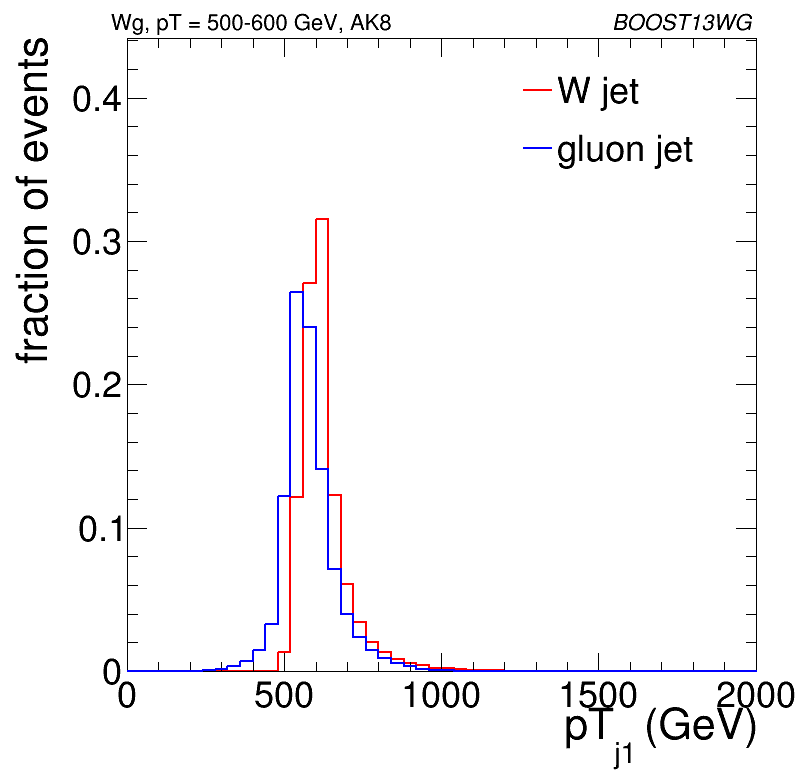
\includegraphics[width=0.30\textwidth]{./Figures/WTagging/pT500/AKtR08/jpt1.png}}
\subfigure[\antikt R=1.2]{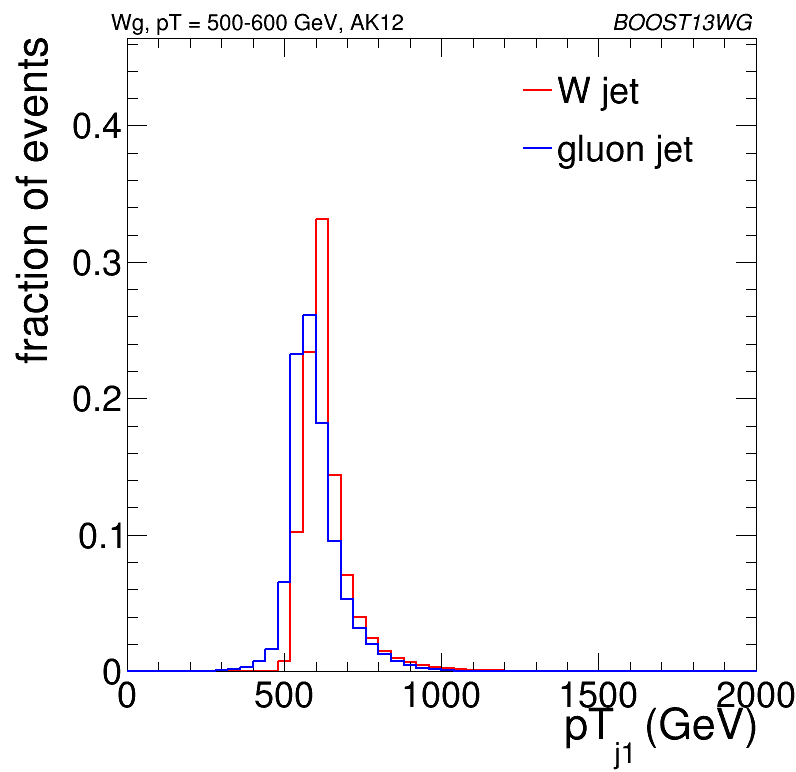
\includegraphics[width=0.30\textwidth]{./Figures/WTagging/pT500/AKtR12/jpt1.png}}
\caption{Comparisons of the leading jet \pt spectrum of the $gg$
  background to the $WW$ signal in the \pt 500-600 GeV parton \pt~slice using the
  different \antikt jet distance parameters explored in this \pt~bin. These
  distributions are formed prior to the 500-600 GeV leading jet \pt~requirement.} 
\label{fig:pt500_basics}
\end{center}
\end{figure*}

\begin{figure*}
\begin{center}
\subfigure[\antikt R=0.4]{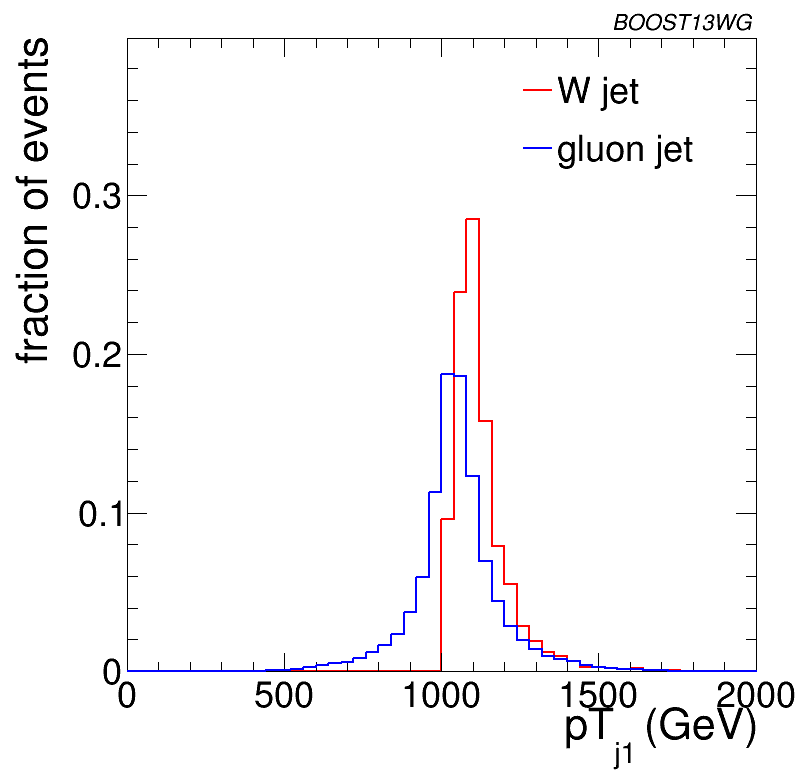
\includegraphics[width=0.30\textwidth]{./Figures/WTagging/pT1000/AKtR04/jpt1.png}}
\subfigure[\antikt R=0.8]{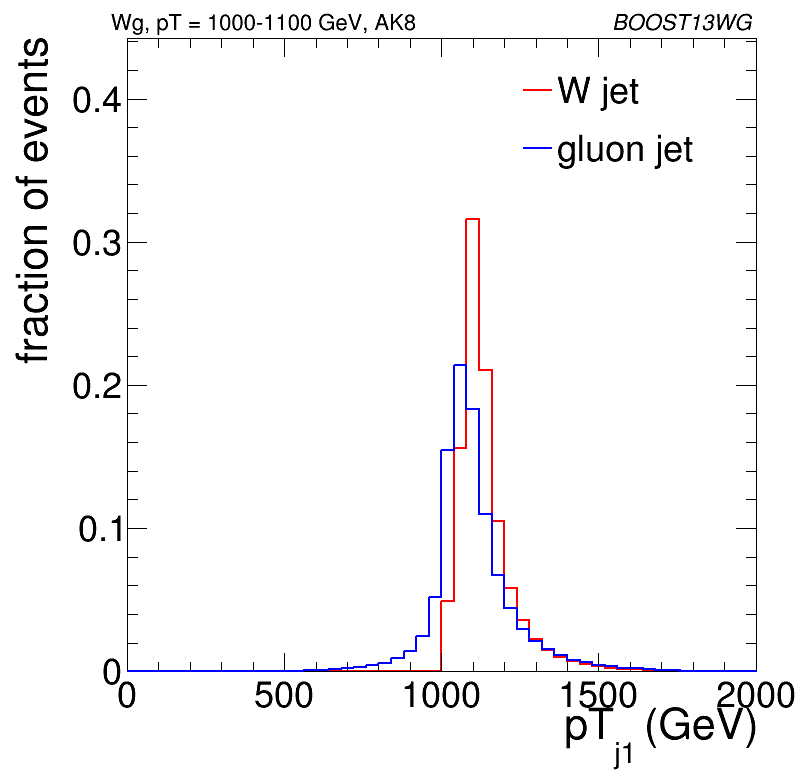
\includegraphics[width=0.30\textwidth]{./Figures/WTagging/pT1000/AKtR08/jpt1.png}}
\subfigure[\antikt R=1.2]{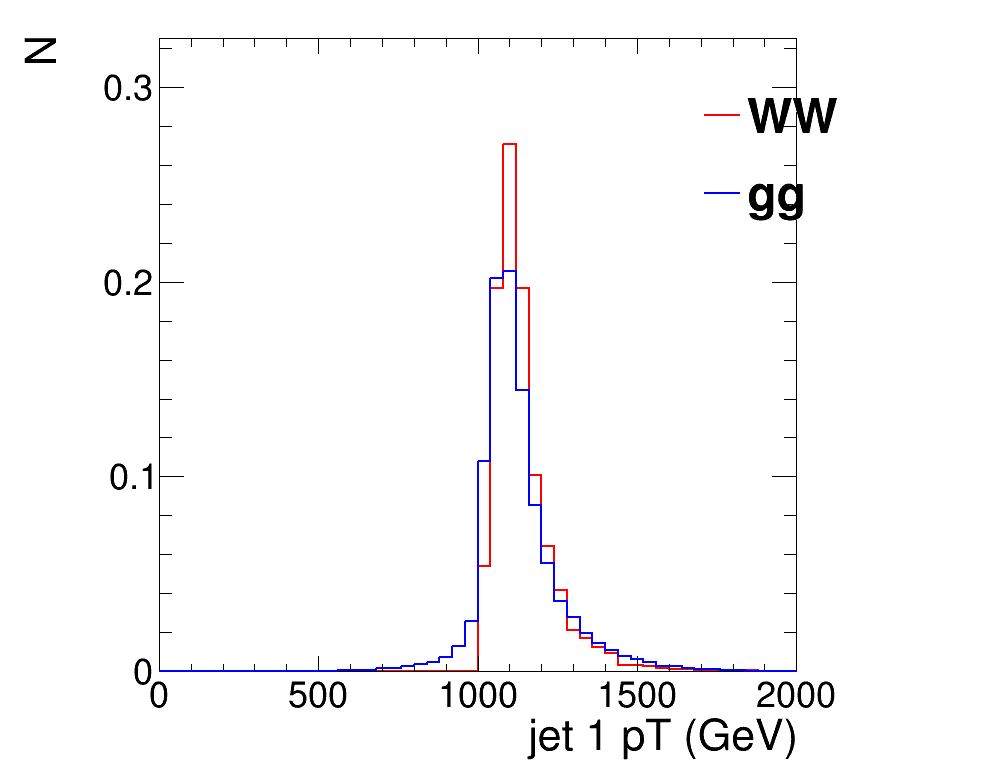
\includegraphics[width=0.30\textwidth]{./Figures/WTagging/pT1000/AKtR12/jpt1.png}}
\caption{Comparisons of the leading jet \pt spectrum of the $gg$
  background to the $WW$ signal in the \pt 1.0-1.1 TeV parton \pt~slice using the
  different \antikt jet distance parameters explored in this \pt~bin. These
  distributions are formed prior to the 500-600 GeV leading jet \pt~requirement.}
\label{fig:pt1000_basics}
\end{center}
\end{figure*}

Figure~\ref{fig:qg_pt500_basics_AKt_R08} shows a comparison of the $\pt$ and $\eta$ distributions of the
 quark and gluon samples with $\pt=500-600$~GeV. 
\begin{figure*}
\begin{center}
\subfigure[Leading jet
\pT]{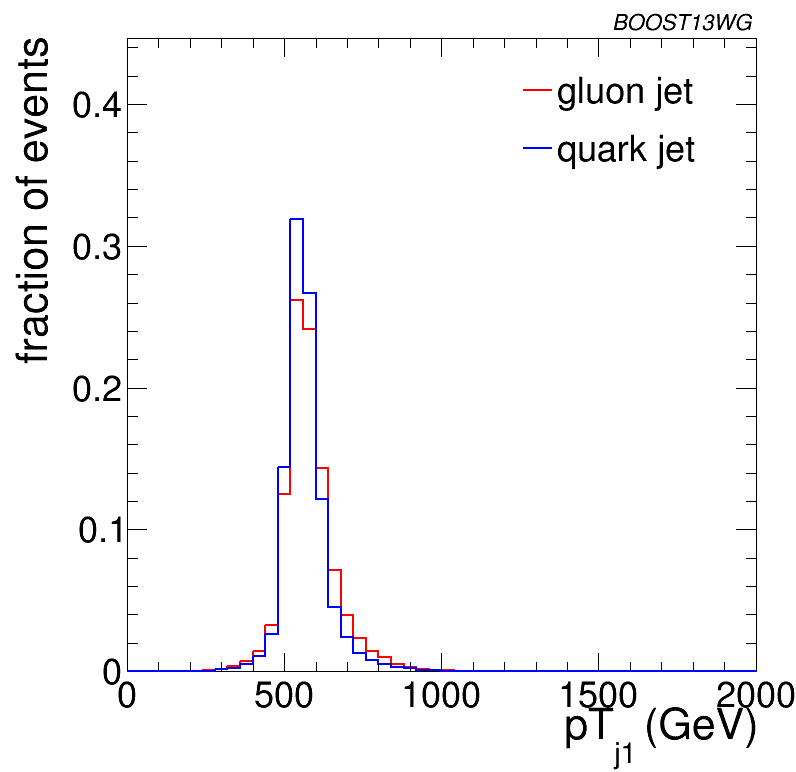
\includegraphics[width=0.40\textwidth]{./Figures/QGTagging/pT500/AKtR08/jpt1.png}}
\subfigure[Sub-leading jet
\pT]{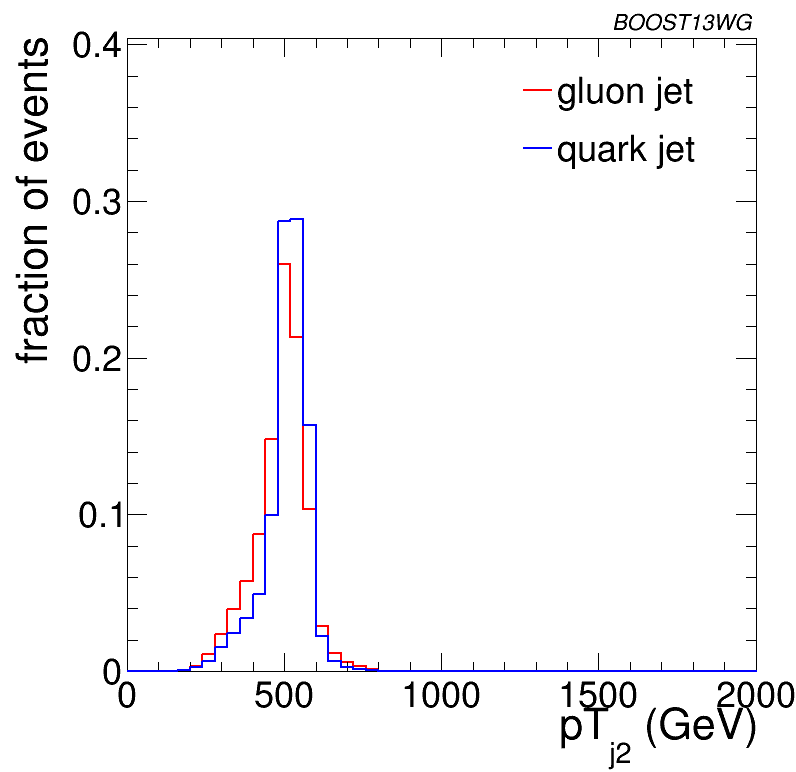
\includegraphics[width=0.40\textwidth]{./Figures/QGTagging/pT500/AKtR08/jpt2.png}}\\
\subfigure[Leading jet
$\eta$]{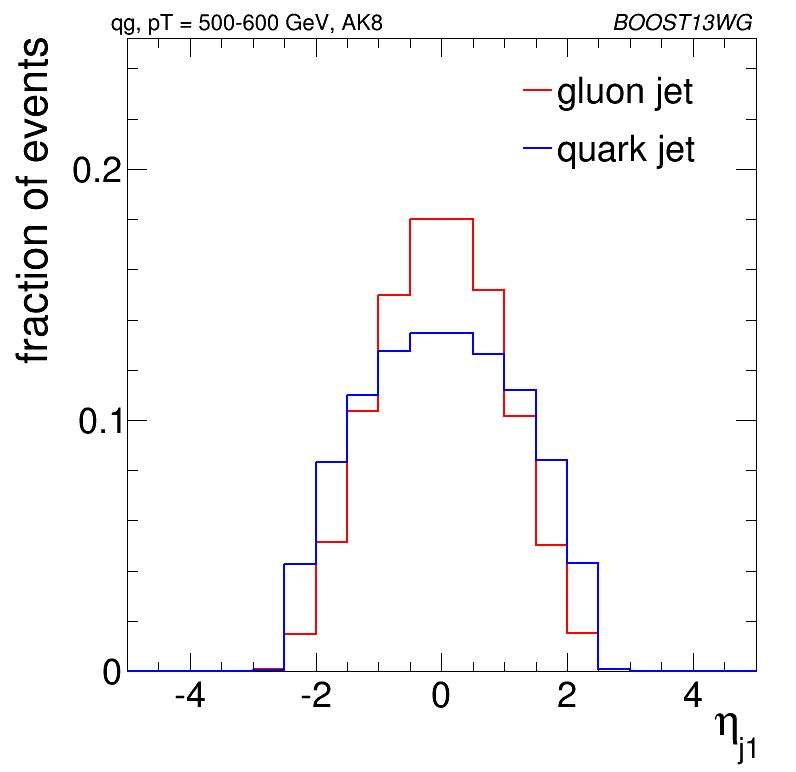
\includegraphics[width=0.40\textwidth]{./Figures/QGTagging/pT500/AKtR08/jeta1.png}}
\subfigure[Sub-leading jet
$\eta$]{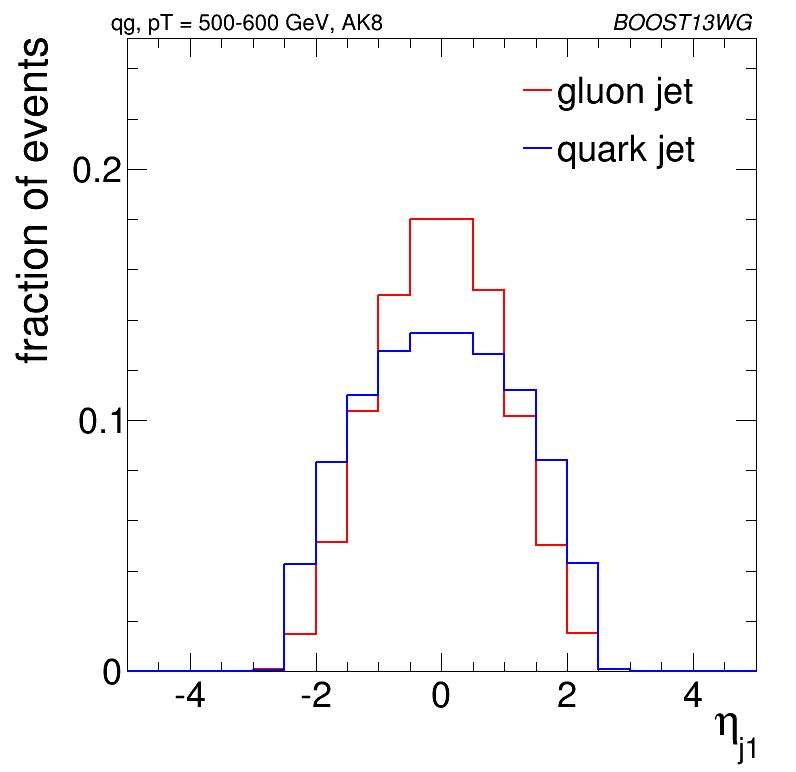
\includegraphics[width=0.40\textwidth]{./Figures/QGTagging/pT500/AKtR08/jeta2.png}}
\caption{Comparisons of quark and gluon $\pt$ and $\eta$ 
distributions in the sample used for the jets of $\pt=500-600 \GeV$ bin using the anti-\kT R=0.8 algorithm.}
\label{fig:qg_pt500_basics_AKt_R08}
\end{center}
\end{figure*}
%
The differences in the $\pt$ distributions can be attributed to different out-of-cone radiation
patterns for quark and gluons; these differences become smaller as the $R$ parameter is increased.
The different $\eta$ distributions are related to the different
parton distribution functions initiating $qq$ and $gg$ production. The qualitative features of the 
$\eta$ distributions do not change as the $R$ parameter is changed. As the $\pt$ increases, 
the $\eta$ distributions peak more strongly near zero, as the probability peaks for processes
initiated by partons of comparable energy. In our analysis, we make a narrow window cut of 100 GeV
 in $\pt$ after showering, and so the effects of the different $q/g$ $\pt$ spectra on our analysis
is suppressed. ({\bf ED: check})

\subsection{Single Variable Discrimination}


Figure~\ref{fig:qg_pt500_mass_AKt_R08} shows the mass of jets in the quark and gluon samples when using
different groomers. Jets built with the anti-\kT algorithm with
R=0.8 and with $\pt=500-650 \GeV$ are used ({\bf BS:Check pT bins in this section!}). 
\begin{figure*}
\begin{center}
\subfigure[Ungroomed mass]{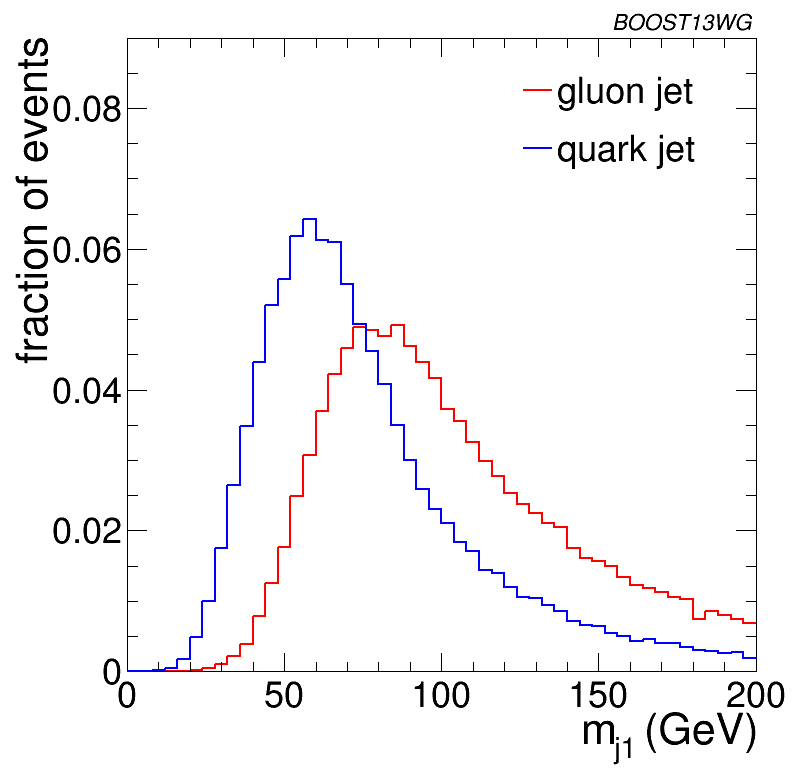
\includegraphics[width=0.30\textwidth]{./Figures/QGTagging/pT500/AKtR08/jmass1.png}}
\subfigure[Pruned mass]{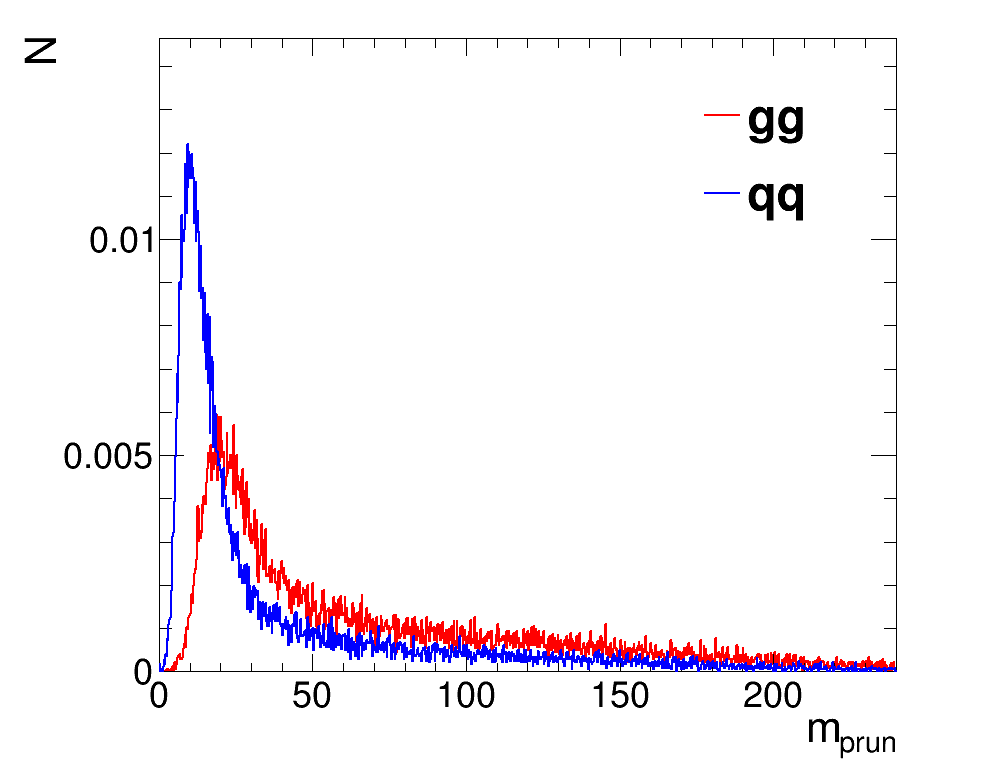
\includegraphics[width=0.30\textwidth]{./Figures/QGTagging/pT500/AKtR08/h_mass_prun.png}}
\subfigure[Trimmed mass]{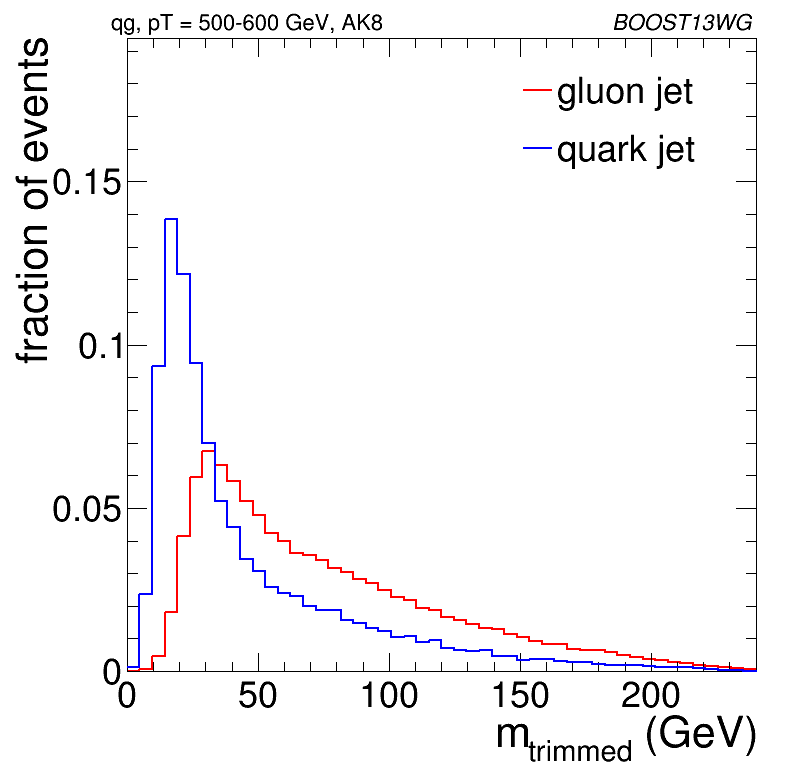
\includegraphics[width=0.30\textwidth]{./Figures/QGTagging/pT500/AKtR08/h_mass_trim.png}}\\
\subfigure[mMDT mass]{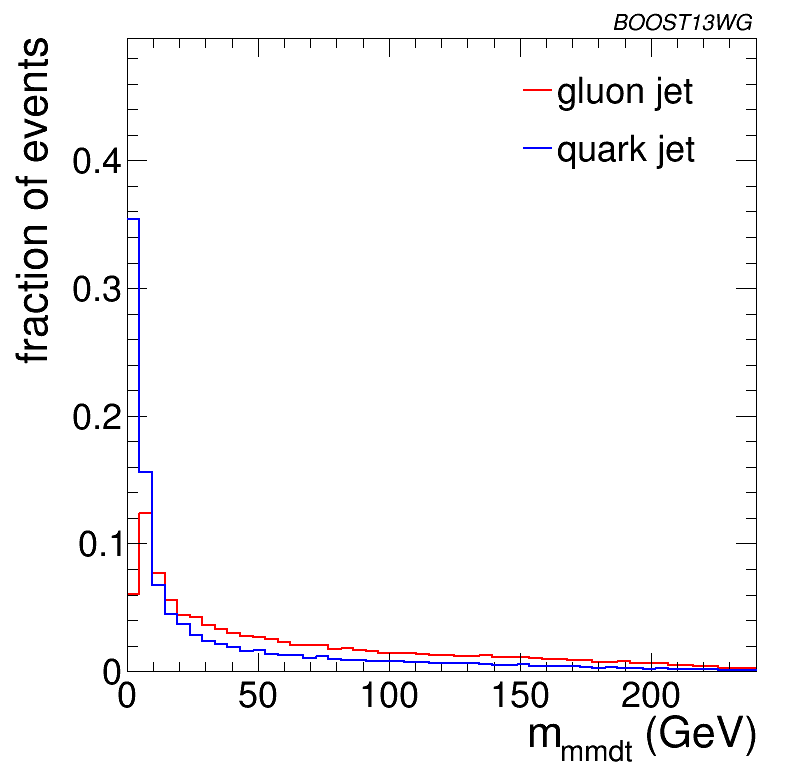
\includegraphics[width=0.30\textwidth]{./Figures/QGTagging/pT500/AKtR08/h_mass_mmdt.png}}
\subfigure[Soft-drop $\beta=2$ mass]{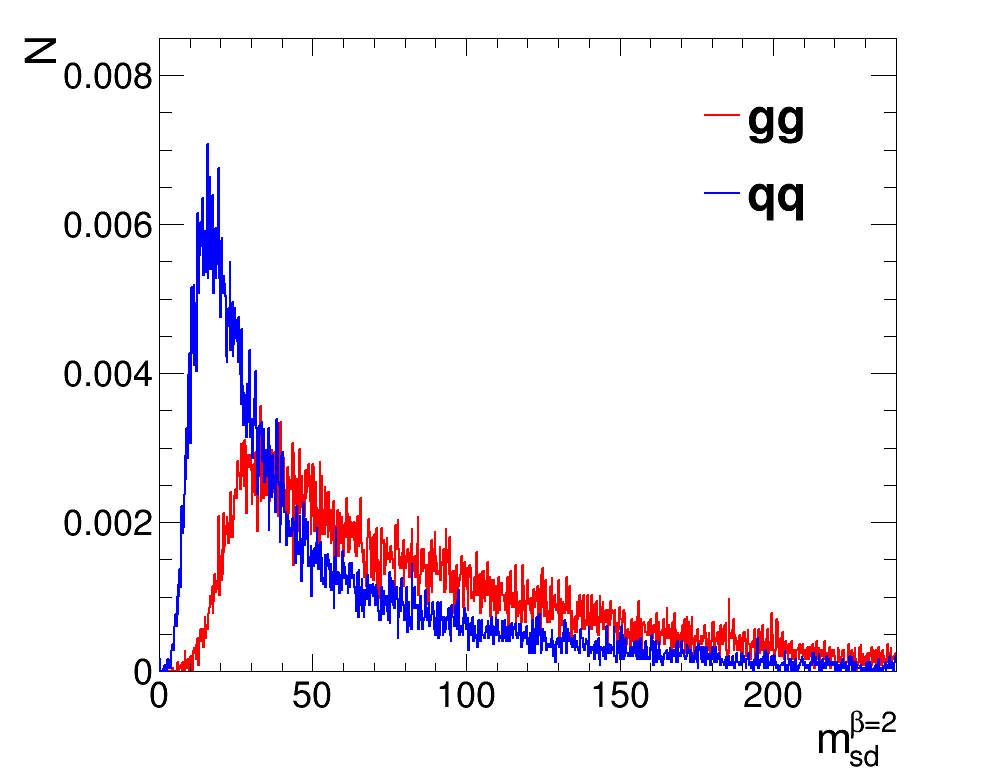
\includegraphics[width=0.30\textwidth]{./Figures/QGTagging/pT500/AKtR08/h_mass_sdb2.png}}
\subfigure[Soft-drop $\beta=-1$ mass]{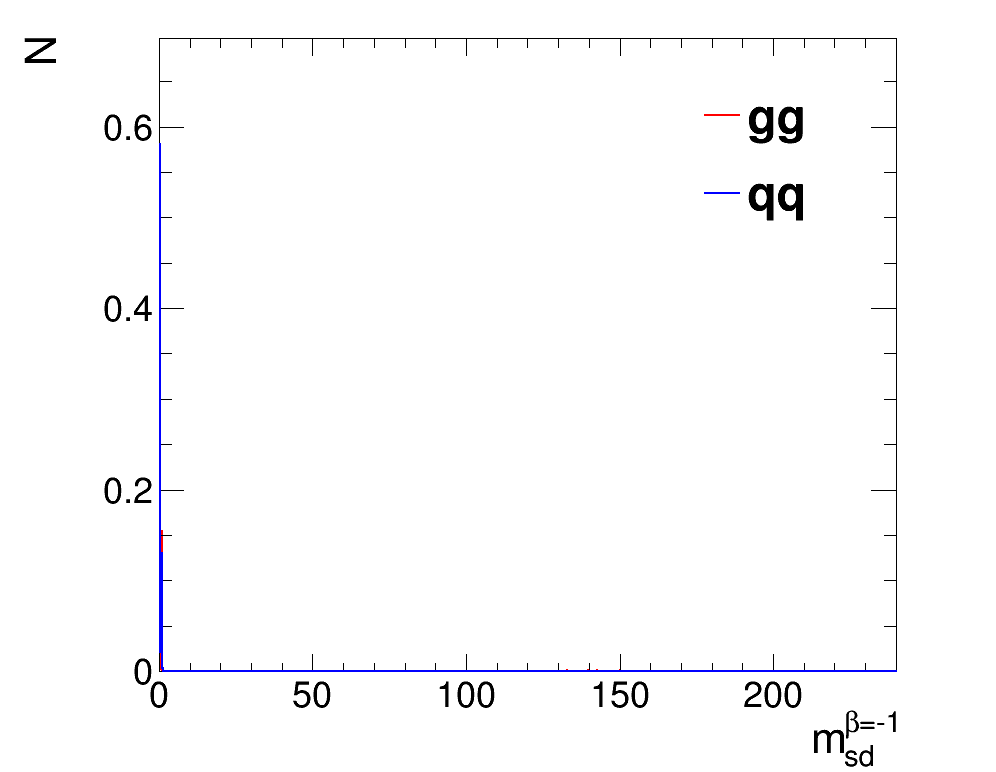
\includegraphics[width=0.30\textwidth]{./Figures/QGTagging/pT500/AKtR08/h_mass_sdm1.png}}
\caption{Comparisons of ungroomed and groomed quark and gluon mass distributions for leading jets in the 
$\pt=500-650 \GeV$ bin using the anti-\kT R=0.8 algorithm. }
\label{fig:qg_pt500_mass_AKt_R08}
\end{center}
\end{figure*}
Qualitatively, the application of grooming shifts the mass distributions towards
lower values as expected. No clear gain in discrimination can be seen, and for
certain grooming parameters, such as the use of soft drop with $\beta=-1$ a clear
loss in discrimination power is observed; this is because the soft-drop condition for $\beta=-1$ discards collinear radiation, and the differences between quarks and gluons are manifest in the collinear structure (spin, splitting functions, etc.). 


\begin{figure*}
\begin{center}
\subfigure[$C_1^{\beta=0}$]{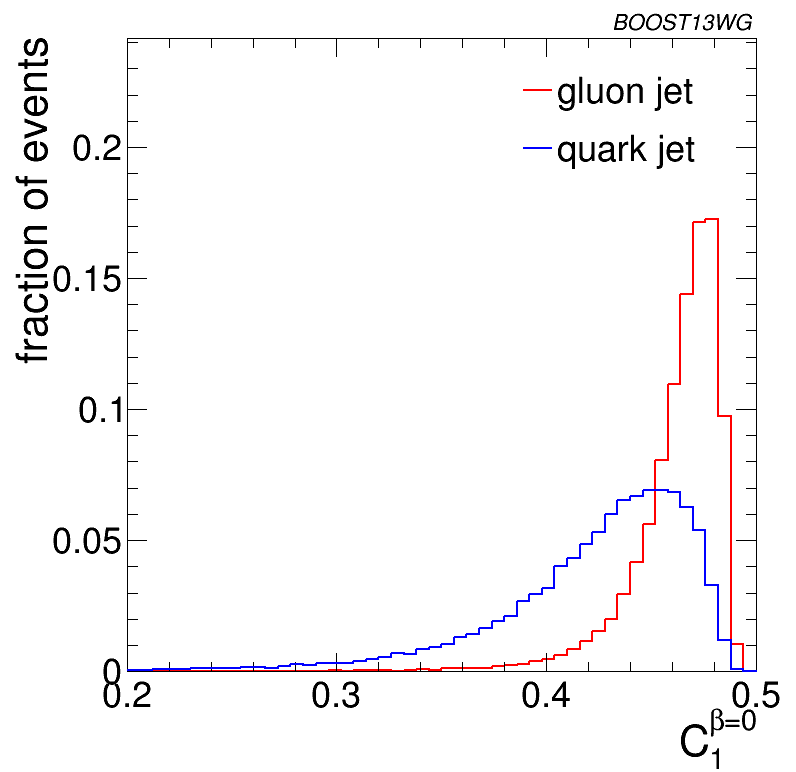
\includegraphics[width=0.30\textwidth]{./Figures/QGTagging/pT500/AKtR08/h_c1_b0.png}}
\subfigure[$C_1^{\beta=1}$]{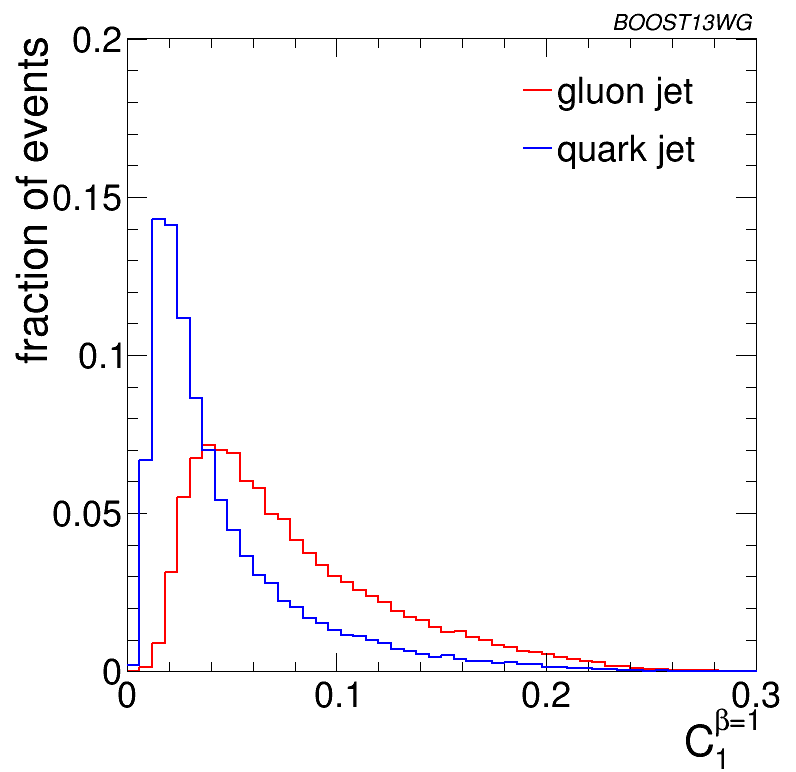
\includegraphics[width=0.30\textwidth]{./Figures/QGTagging/pT500/AKtR08/h_c1_b1.png}}
\subfigure[$C_1^{\beta=2}$]{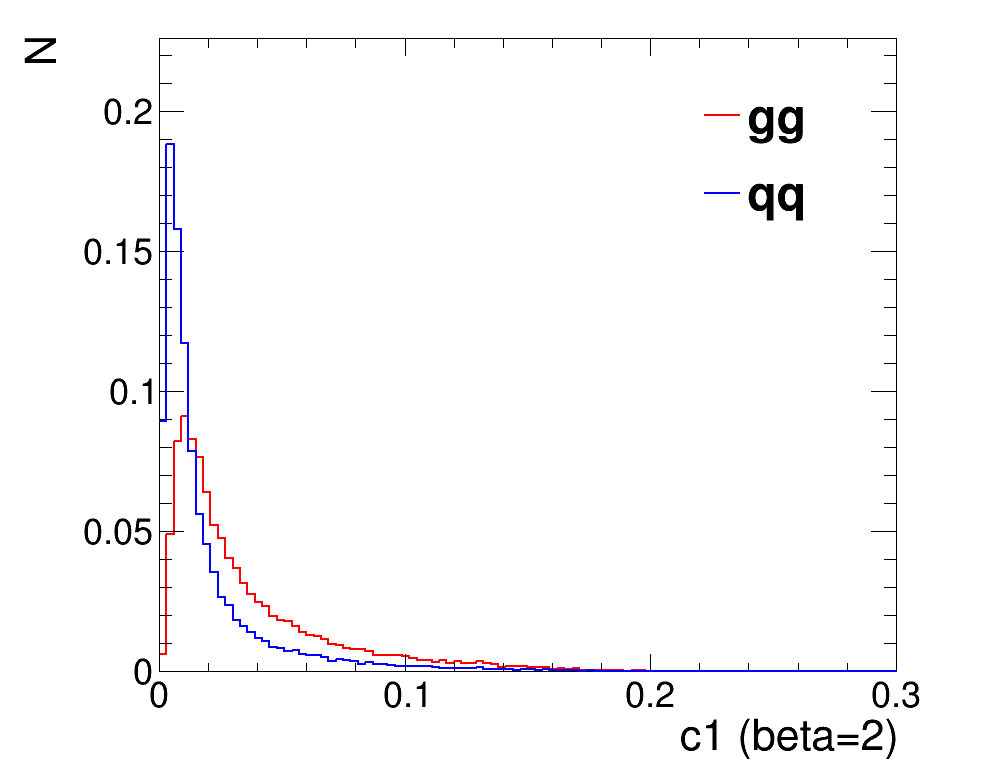
\includegraphics[width=0.30\textwidth]{./Figures/QGTagging/pT500/AKtR08/h_c1_b2.png}}\\
\subfigure[$\Gamma_{Qjet}$]{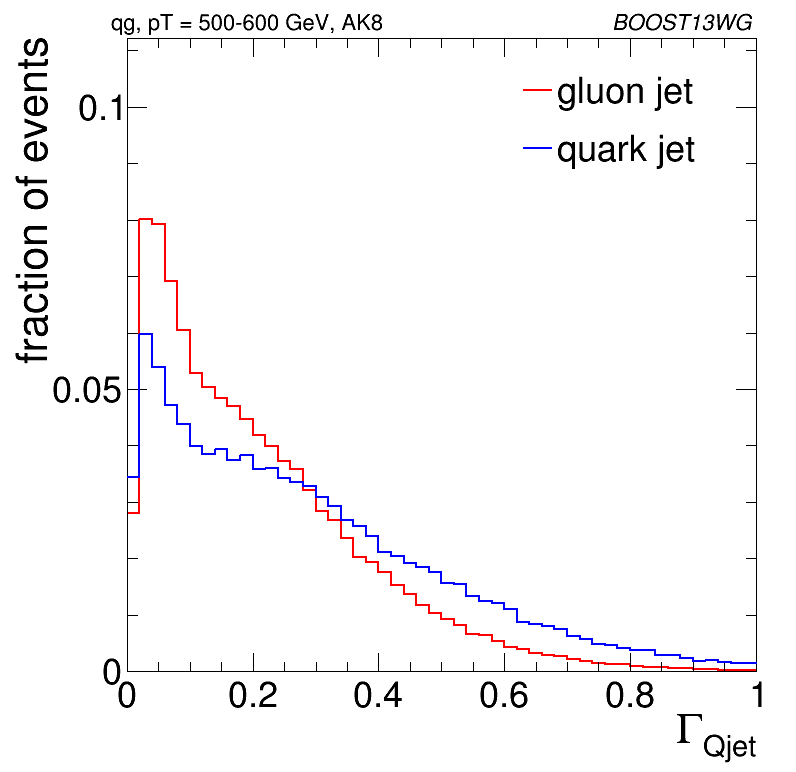
\includegraphics[width=0.30\textwidth]{./Figures/QGTagging/pT500/AKtR08/h_qjetVol.png}}
\subfigure[$\rm{n_ {constits}}$]{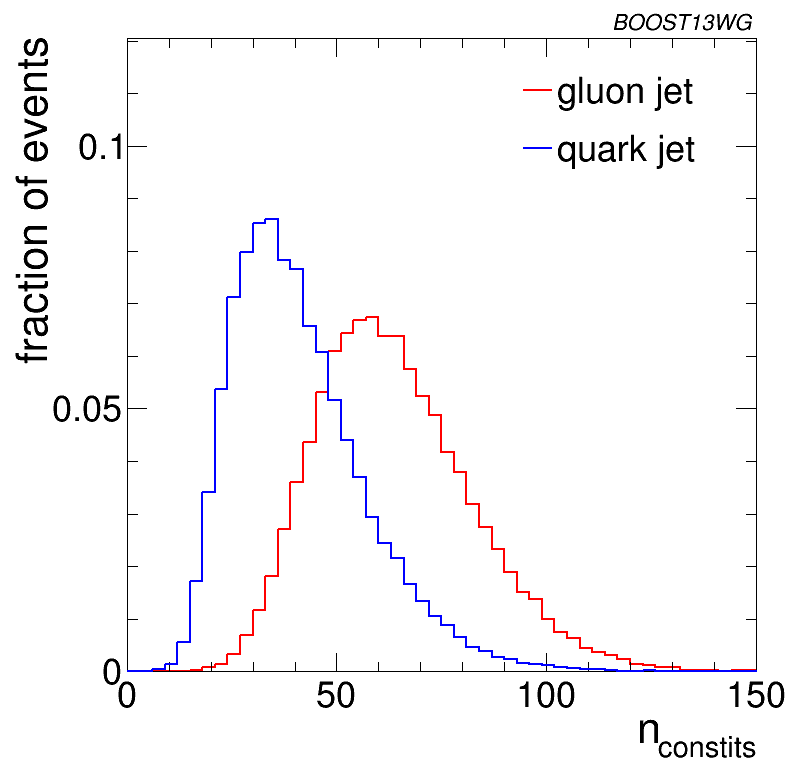
\includegraphics[width=0.30\textwidth]{./Figures/QGTagging/pT500/AKtR08/h_multiplicity.png}}
\subfigure[$\tau_{1}^{\beta=1}$]{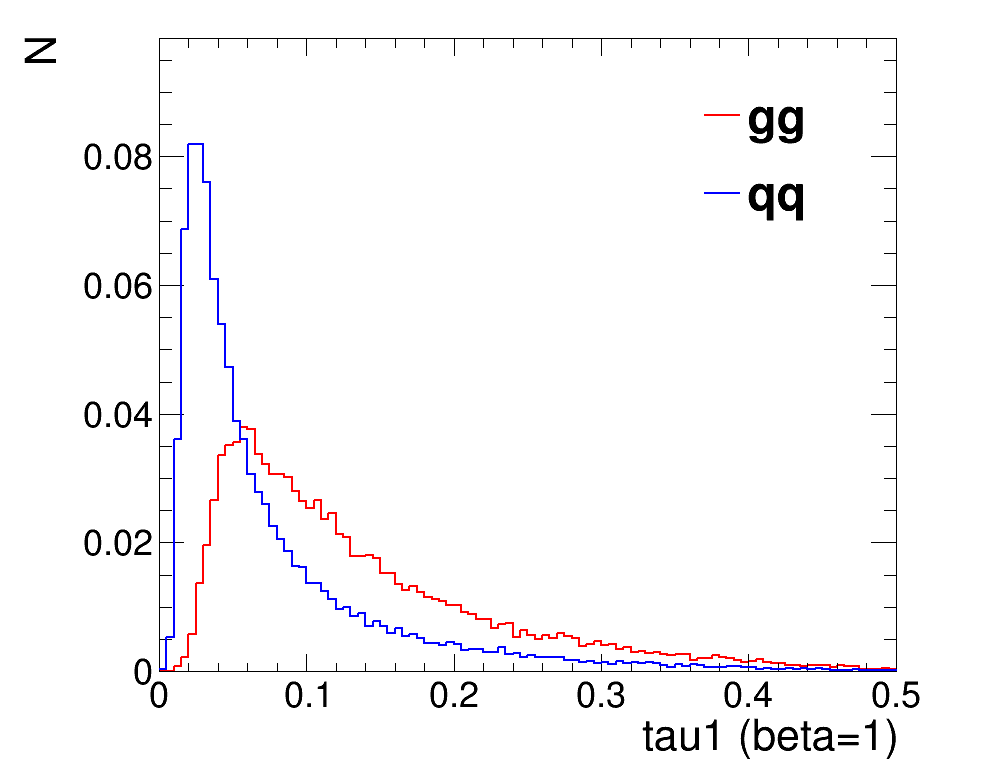
\includegraphics[width=0.30\textwidth]{./Figures/QGTagging/pT500/AKtR08/h_tau1_b1.png}}\\
\subfigure[$\tau_{1}^{\beta=2}$]{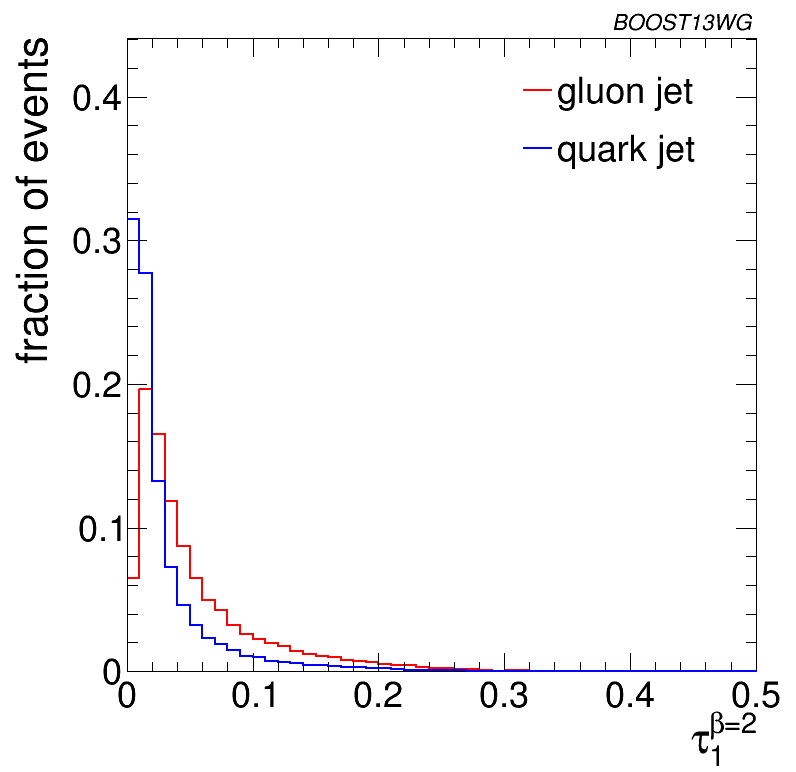
\includegraphics[width=0.30\textwidth]{./Figures/QGTagging/pT500/AKtR08/h_tau1_b2.png}}
\caption{Comparisons of quark and gluon distributions of different substructure variables for leading jets in the 
$\pt=500-650 \GeV$ bin using the anti-\kT R=0.8 algorithm. }
\label{fig:qg_pt500_subst_AKt_R08}
\end{center}
\end{figure*}

The performance of different substructure variables is explored in Figure~\ref{fig:qg_pt500_subst_AKt_R08}. Among those considered, $n_{\rm constits}$ provides the highest separation
power, followed by $C_1^{\beta=0}$ and $C_1^{\beta=1}$ as was also found by the CMS and ATLAS Collaborations\refneeded.

To more quantitatively study the power of each observable as a
discriminator for quark/gluon tagging, Receiver Operating Characteristic (ROC) curves are built by scanning each distribution
and plotting the background efficiency (to select gluon jets) vs.~the signal efficiency (to select quark jets). 
Figure~\ref{fig:qg_pt300_single} shows these ROC curves for all of the variables shown in 
Figure~\ref{fig:qg_pt500_subst_AKt_R08} and the ungroomed mass, representing the 
best performing mass variable, for jets of $\pt=300-400\GeV$. In addition, we show the ROC curve for 
the tagger built from a BDT combining all the variables. The details of how the BDT is constructed 
are explained in Section~\ref{sec:multivariate}. 
%
\begin{figure*}
\begin{center}
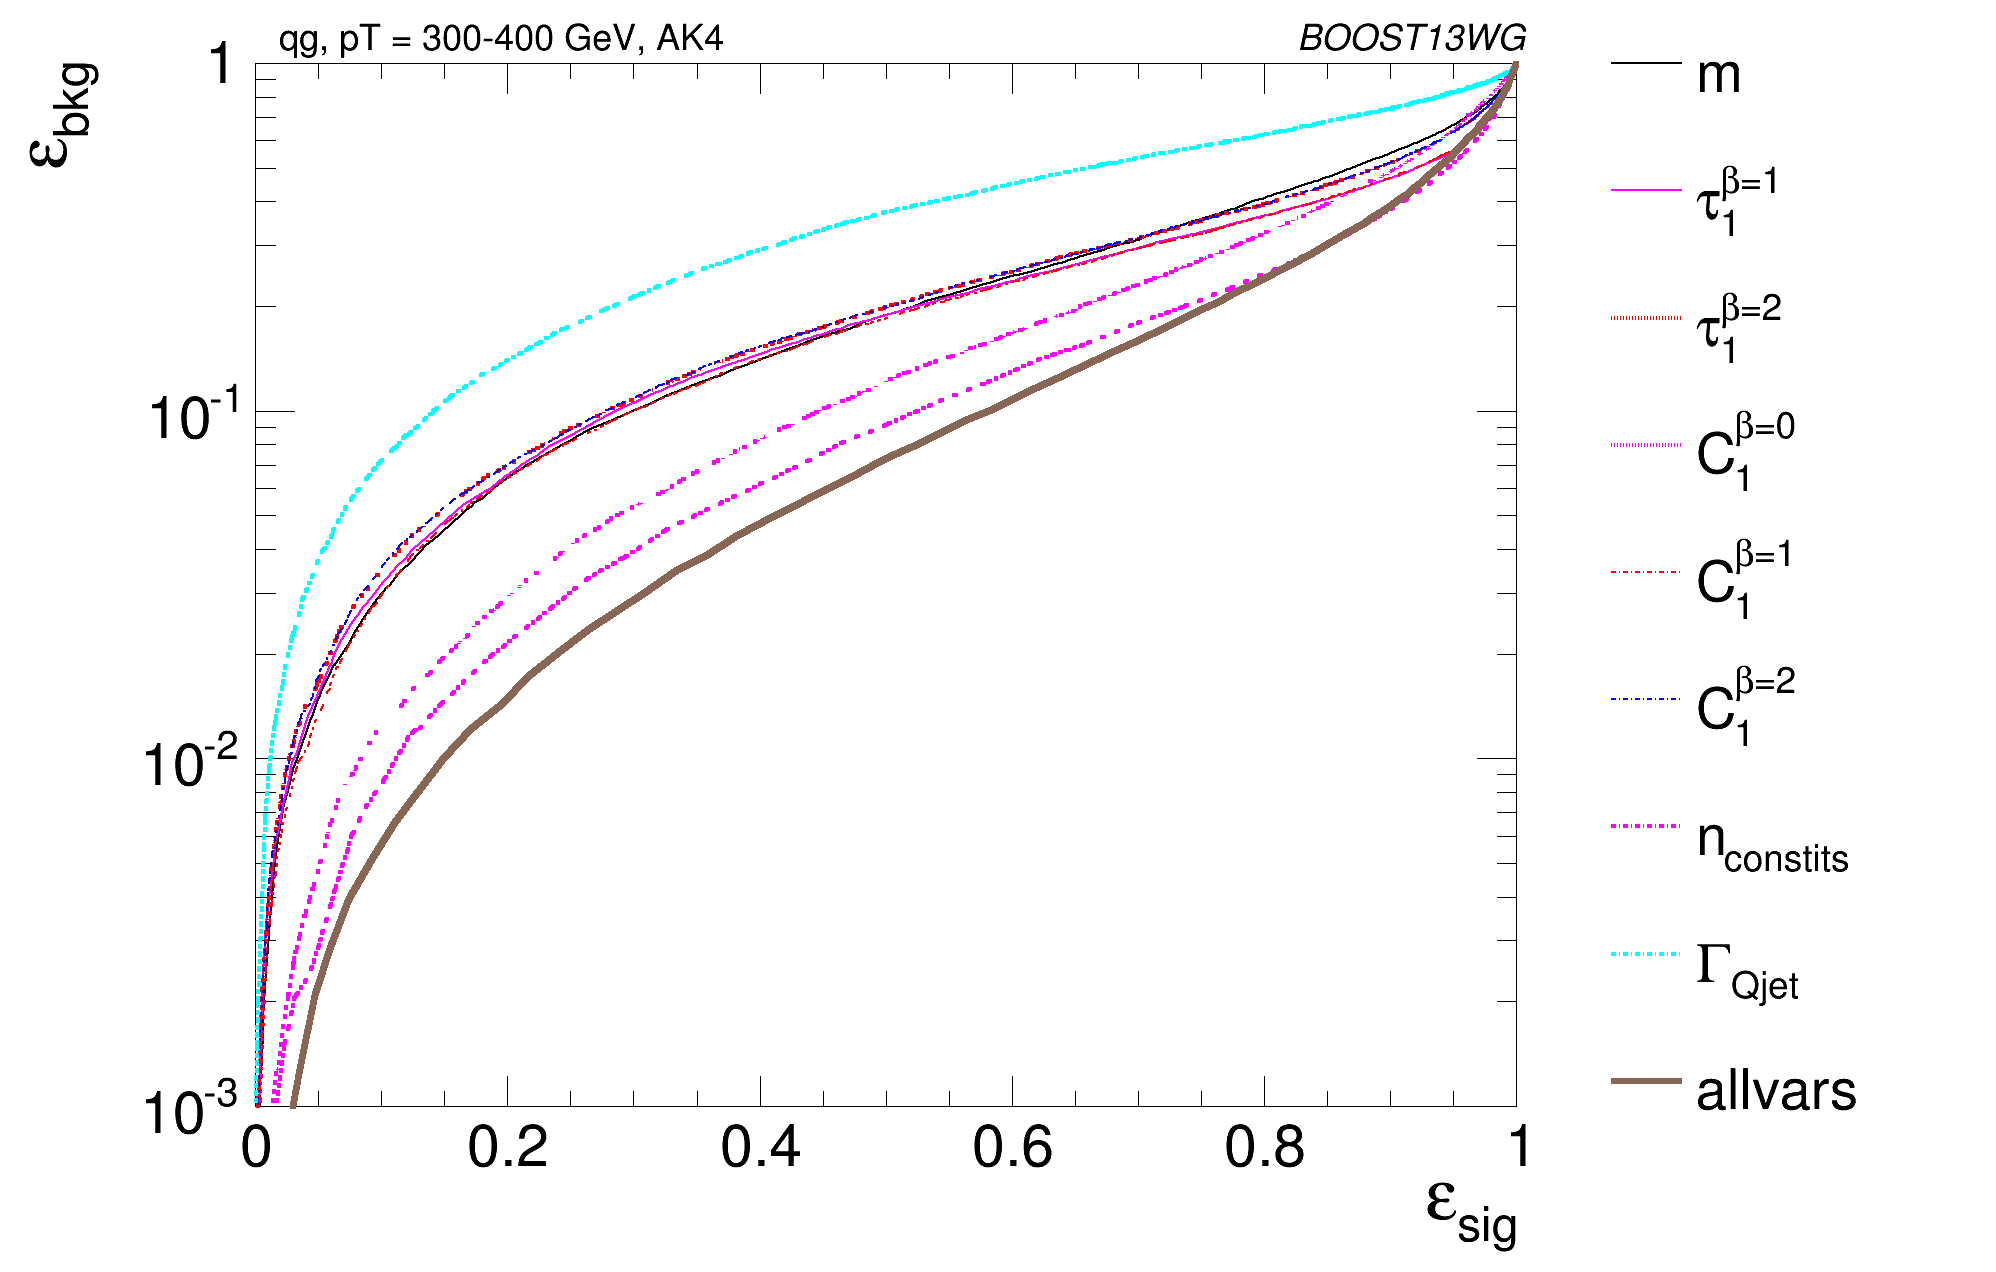
\includegraphics[width=0.32\textwidth]{./Figures/QGTagging/pT300/AKtR04/Rocs_1D_single.png}
%\includegraphics[width=0.4\textwidth]{./Figures/QGTagging/pT1000/AKtR04/Rocs_1D_single.png}\\
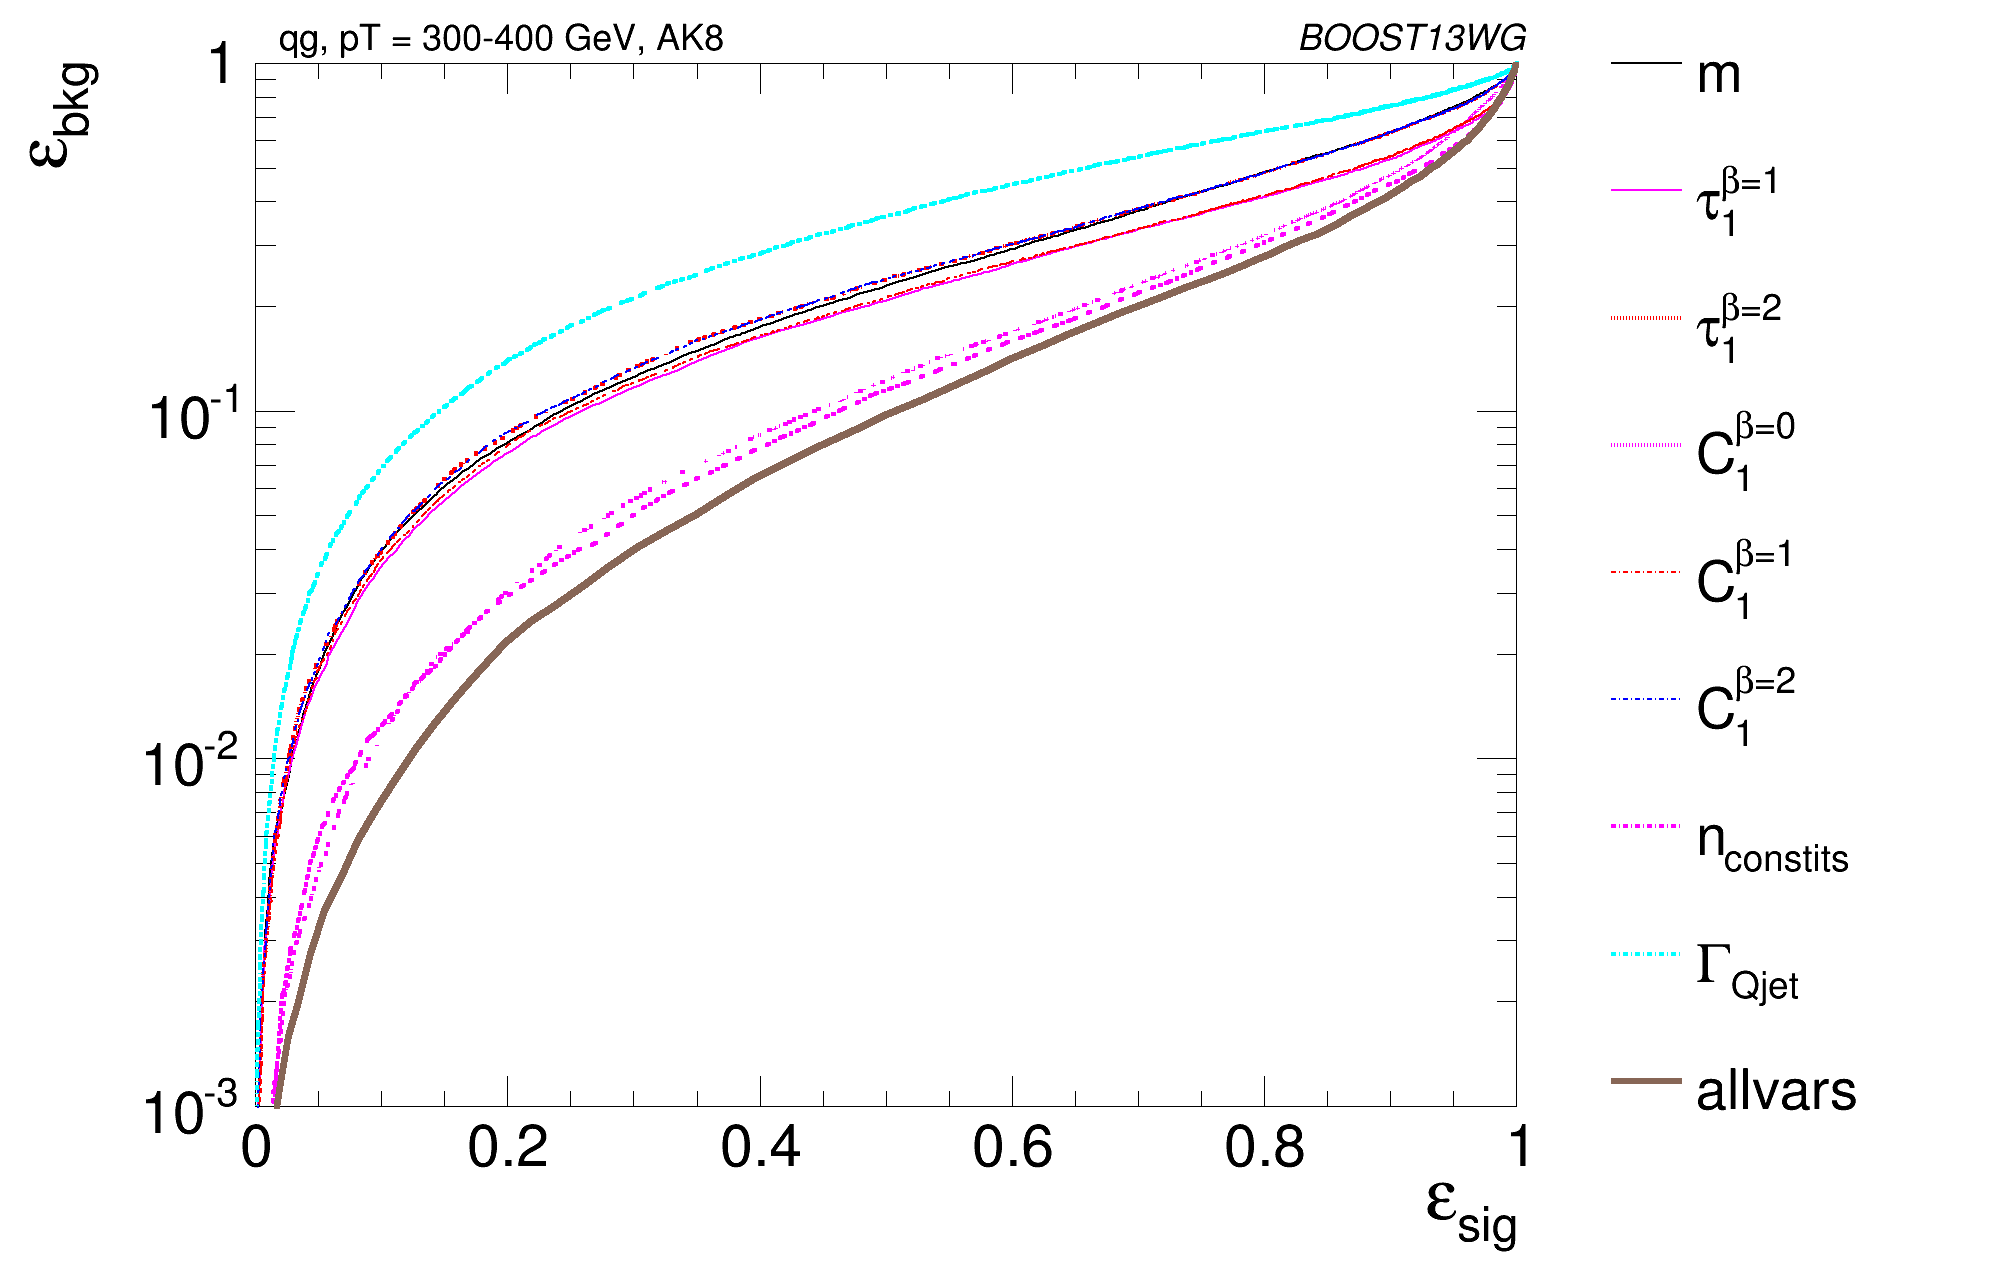
\includegraphics[width=0.32\textwidth]{./Figures/QGTagging/pT300/AKtR08/Rocs_1D_single.png}
%\includegraphics[width=0.4\textwidth]{./Figures/QGTagging/pT1000/AKtR08/Rocs_1D_single.png}\\
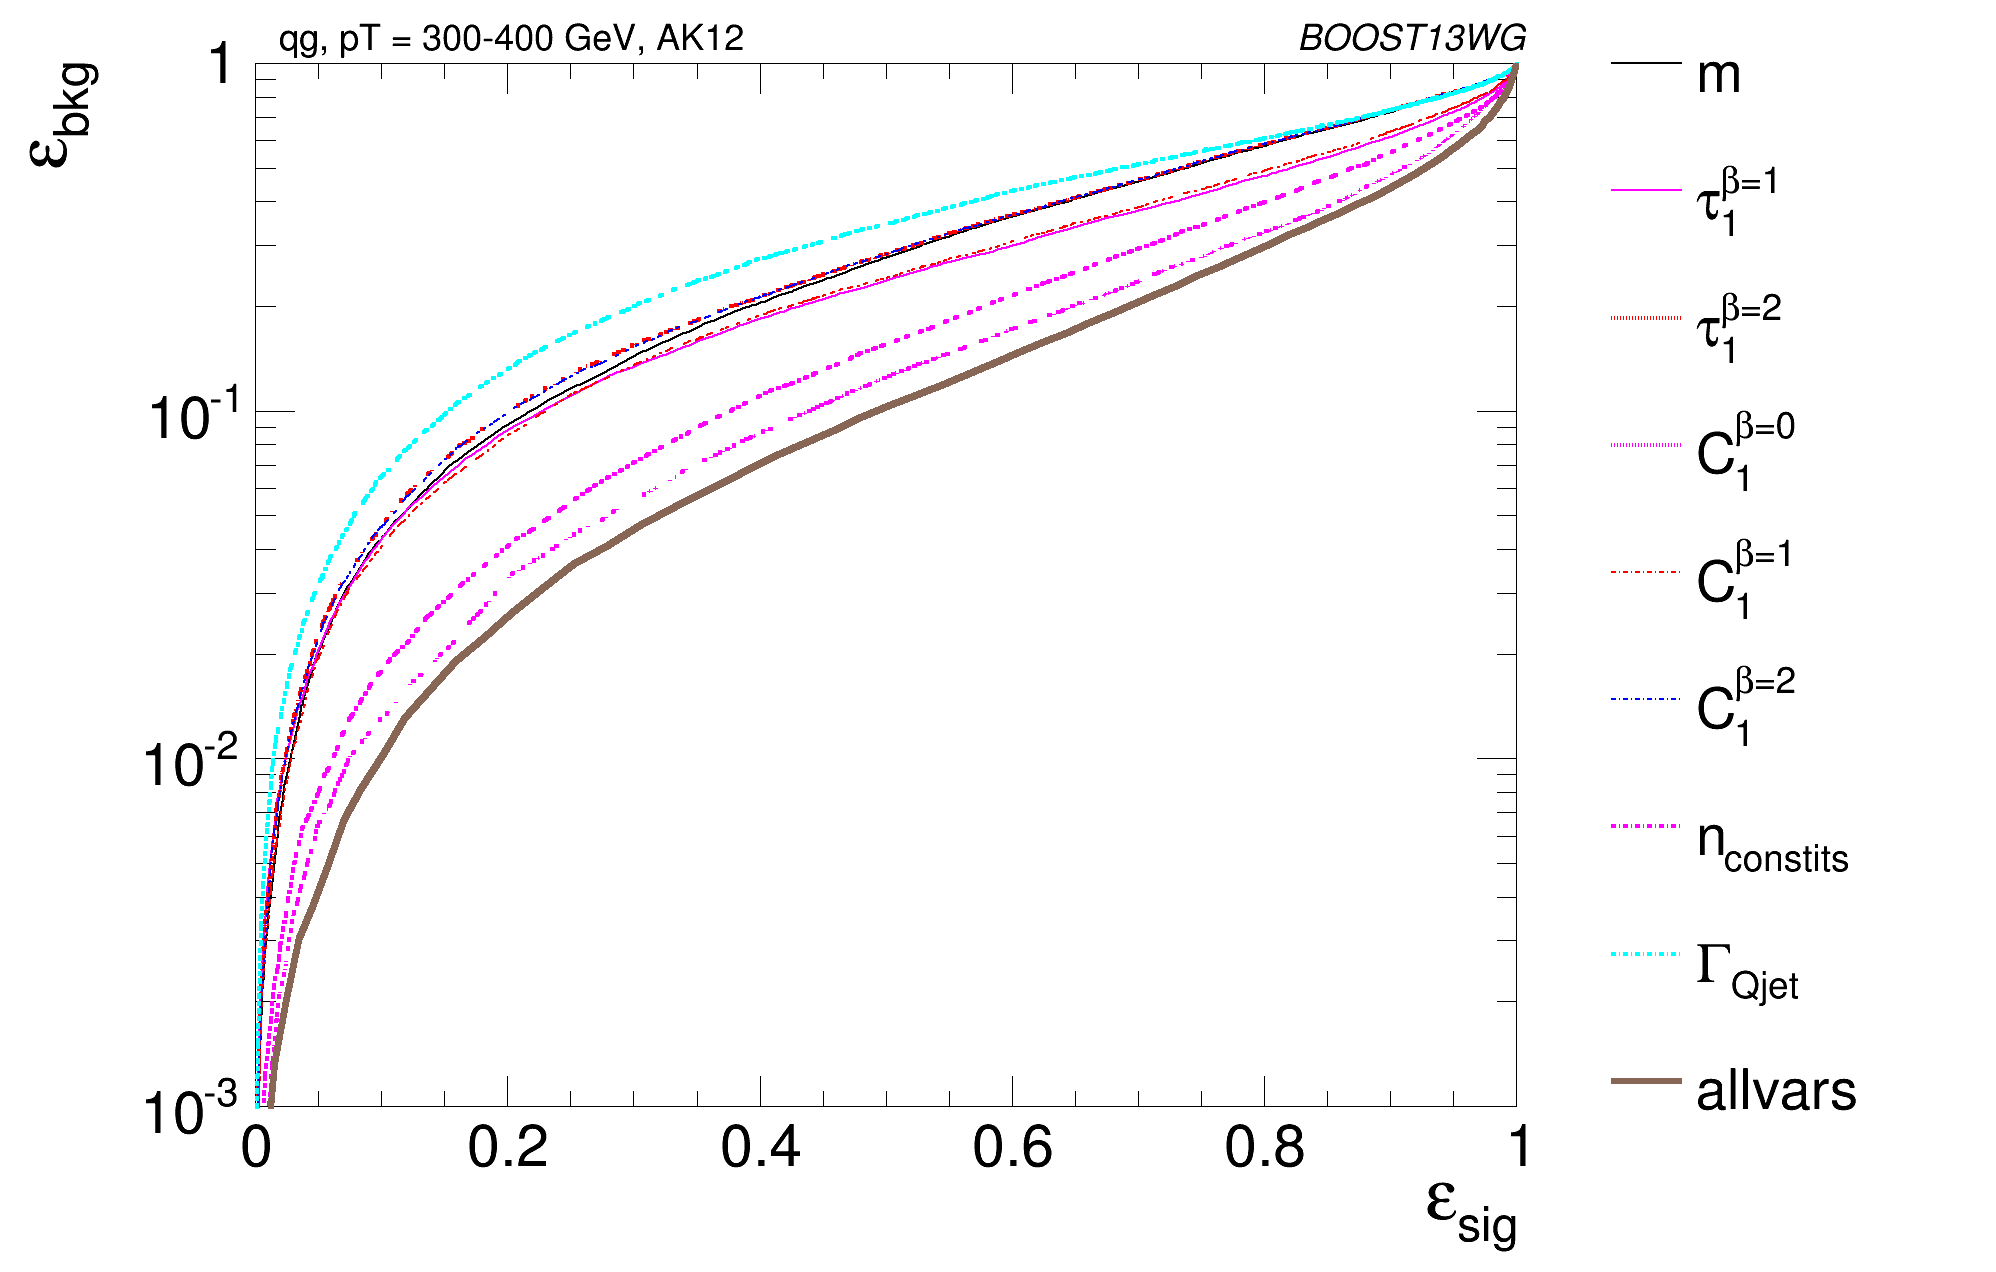
\includegraphics[width=0.32\textwidth]{./Figures/QGTagging/pT300/AKtR12/Rocs_1D_single.png}
%\includegraphics[width=0.4\textwidth]{./Figures/QGTagging/pT1000/AKtR12/Rocs_1D_single.png}\\
\caption{The ROC curve for all single variables considered for quark-gluon discrimination in the \pt 500 GeV bin using the anti-\kT R=0.8 algorithm.}
\label{fig:qg_pt300_single}
\end{center}
\end{figure*}
%
Clearly, $n_{\rm constits}$ is the best performing variable for all Rs, even though $C_1^{\beta=0}$ is close, particularly
for R=0.8. Most other variables have similar performance, except the Q-jet volatility, which shows significantly worse
discrimination (this may be due to our choice of
rigidity $\alpha = 0.1$, while other studies suggest that a smaller value,
such as $\alpha = 0.01$, produces better results). The combination of all variables shows somewhat better discrimination.

We now examine how performance of masses and substructure observables changes with $\pt$ and $R$. For jet masses, few variations are observed as the 
radius parameter of the jet reconstruction is increased in the two highest $\pt$ bins; this is because the radiation
is more collimated and the dependence on $R$ is consequently smaller.
However, for the $300-400\GeV$ bin, the use of small-$R$ jets produces a shift in the
mass distributions towards lower values, so that large-$R$ jet masses are more stable
with $\pt$ and small-$R$ jet masses are smaller at low-$\pt$ as expected from the spatial
constraints imposed by the $R$ parameter. These statements are explored more 
quantitatively later in this section. ({\bf BS: Do we have plots for this?})

The evolution of some of the substructure variable distributions with $\pt$ and R is less trivial than
 for the jet masses. In particular, changing the $R$ parameter at high $\pt$ changes significantly the $C_a^{\beta}$
for $\beta>0$ and the $n_{\rm constits}$ distributions, while leaving all other distributions qualitatively unchanged. 
This is illustrated in Figure~\ref{fig:Rdep_qg_C_pt1000} for $\beta=0$ and $\beta=1$ using $a=1$ in both cases for
jets with $\pt=1-1.2\TeV$. 

 %
\begin{figure*}
\begin{center}
\subfigure[$C_1^{\beta=0}$, $R=0.4$]{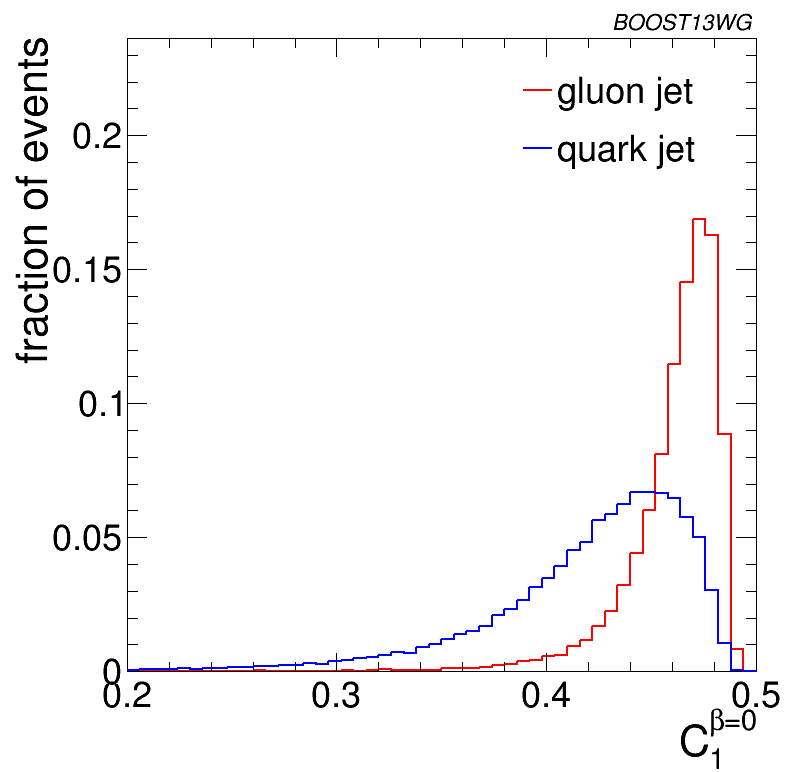
\includegraphics[width=0.30\textwidth]{./Figures/QGTagging/pT1000/AKtR04/h_c1_b0.png}}
\subfigure[$C_1^{\beta=0}$, $R=0.8$]{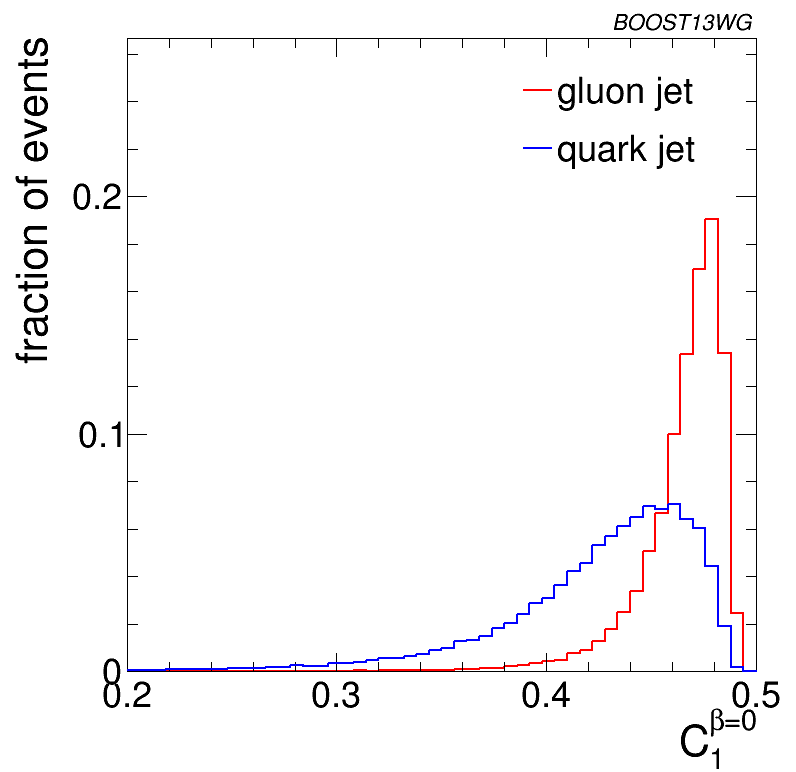
\includegraphics[width=0.30\textwidth]{./Figures/QGTagging/pT1000/AKtR08/h_c1_b0.png}}
\subfigure[$C_1^{\beta=0}$, $R=1.2$]{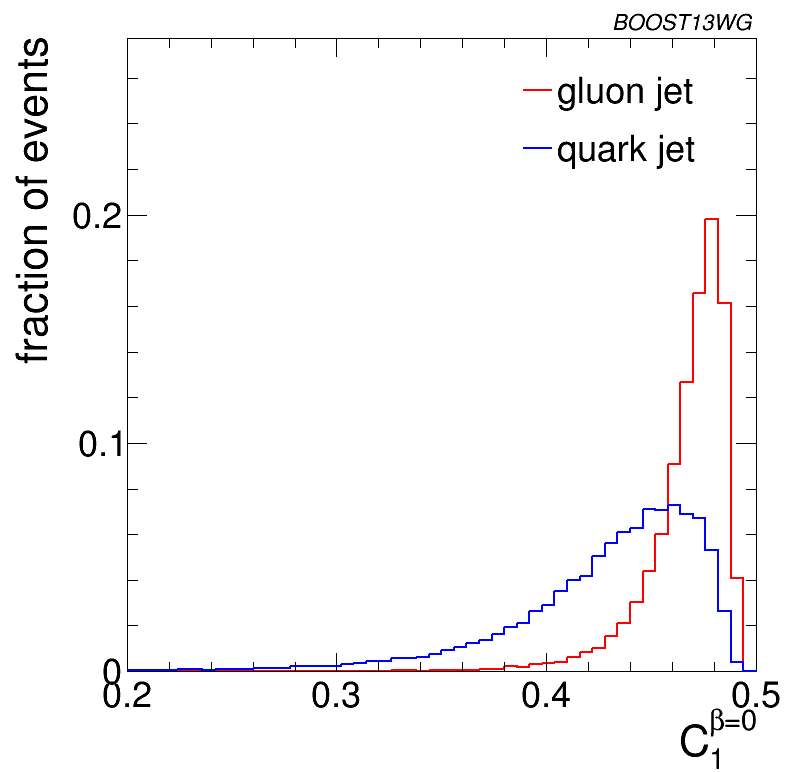
\includegraphics[width=0.30\textwidth]{./Figures/QGTagging/pT1000/AKtR12/h_c1_b0.png}}\\
\subfigure[$C_1^{\beta=1}$, $R=0.4$]{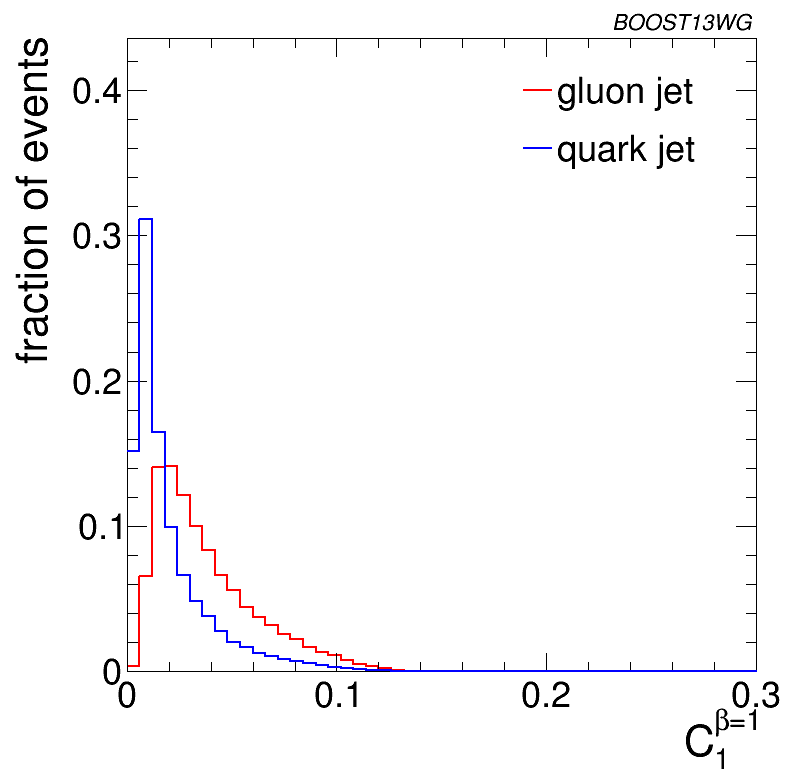
\includegraphics[width=0.30\textwidth]{./Figures/QGTagging/pT1000/AKtR04/h_c1_b1.png}}
\subfigure[$C_1^{\beta=1}$, $R=0.8$]{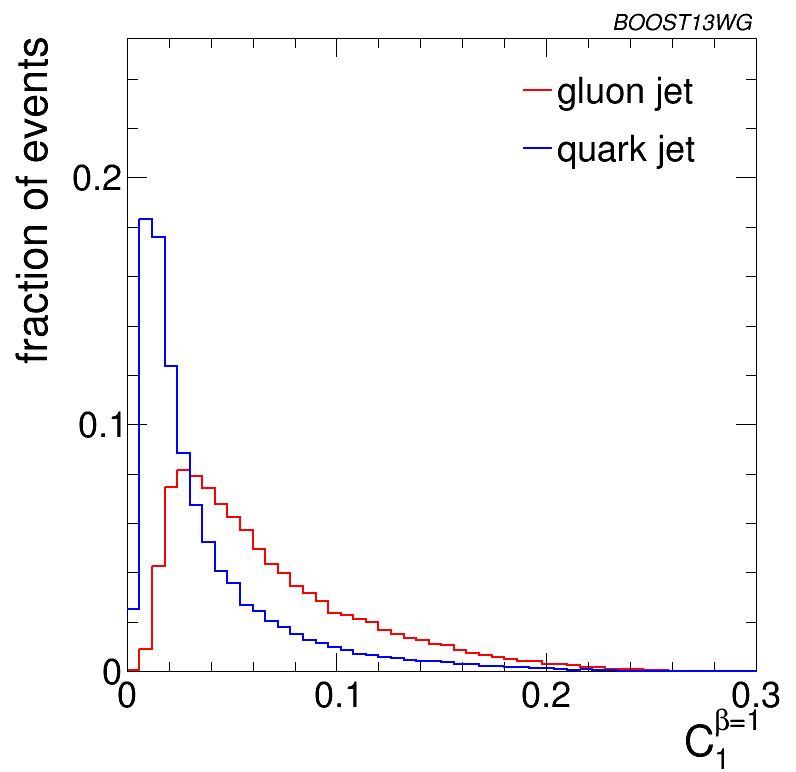
\includegraphics[width=0.30\textwidth]{./Figures/QGTagging/pT1000/AKtR08/h_c1_b1.png}}
\subfigure[$C_1^{\beta=1}$, $R=1.2$]{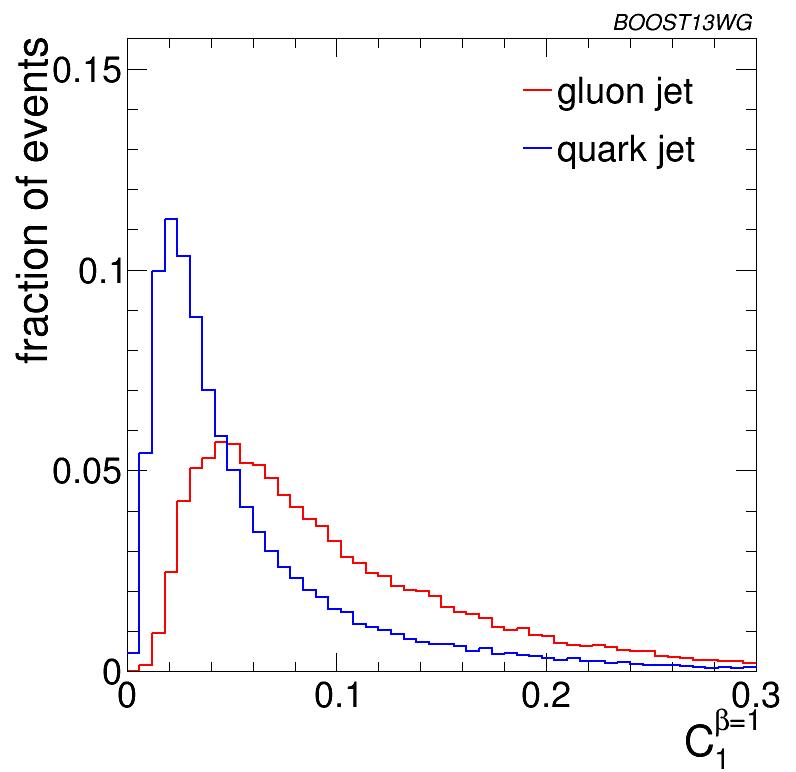
\includegraphics[width=0.30\textwidth]{./Figures/QGTagging/pT1000/AKtR12/h_c1_b1.png}}\\
\caption{Comparisons of quark and gluon distributions of $C_1^{\beta=0}$ (top) and $C_1^{\beta=1}$ (bottom) 
for leading jets in the $\pt=1-1.2 \TeV$ bin using the anti-\kT algorithm with $R=0.4$, 0.8 and 1.2. }
\label{fig:Rdep_qg_C_pt1000}
\end{center}
\end{figure*}
The shift towards lower values with changing R is evident for the $C_1^{\beta=1}$ distributions, while the stability
of $C_1^{\beta=0}$ can also be observed. These features are present in all $\pt$ bins studied, but are even more
pronounced for lower $\pt$ bins. The shape of the Q-jet volatility distribution shows some non-trivial shape that
deserves some explanation. Two peaks are observed, one at low volatility values and one at mid-volatility. These
peaks are generated by two somewhat distinct populations. The high volatility peak arises from jets that get their
mass primarily from soft (and sometimes wide-angle) emissions. The removal of some of the constituents when
building Q-jets thus changes the mass significantly, increasing the volatility. The lower volatility peak corresponds
to jets for which mass is generated by a hard emission, which makes the fraction of Q-jets that change 
the mass significantly to be smaller. Since the probability of a hard emission is proportional to the colour
charge (squared),  the volatility peak is higher for gluon jets by about the colour factor $C_A/C_F$. 



In summary, the overall discriminating power between quarks and gluons
 decreases with increasing R due to the reduction in the amount of out-of-cone radiation differences and 
 and increased contamination from the underlying event ({\bf BS: is this ok?}). The broad performance features discussed for this $\pt$ bin also apply to the higher
$\pt$ bins. These  is further quantified in the next section. 


\subsection{Combined Performance and Correlations}\label{sec:qg_combi}
The quark/gluon tagging performance can be further improved over cuts on single observables by 
combining multiple observables in a BDT; due to the challenging nature of $q$/$g$-tagging, any
improvement in performance with multivariable techniques could be critical for certain analyses, and the 
improvement could be more substantial in data than the marginal benefit found in MC  and shown
in Fig.~\ref{fig:qg_pt300_single}.
 Furthermore, insight can be gained into the 
features allowing for quark/gluon discrimination if the origin of the improvement  is
understood. To quantitatively study this improvement, we build quark/gluon taggers from
every pair-wise combination of variables studied in the previous section for comparison
with the all-variable combination. 

In order to quantitatively study the value of each variable for quark/gluon tagging, we study the gluon 
rejection, defined as $1/\epsilon_{\rm gluon}$, at a fixed quark selection efficiency
of 50\% using jets with $\pt=1-1.2 \TeV$ and for different $R$ parameters. Figure~\ref{fig:qg_pt1000_comb} shows the gluon rejection for each pair-wise combination. 
The pair-wise gluon rejection at 50\% quark efficiency can be compared to the single-variable
values shown along the diagonal. The gluon rejection for the 
BDT all-variable combination is also shown on the bottom right of each plot.
\begin{figure*}
\begin{center}
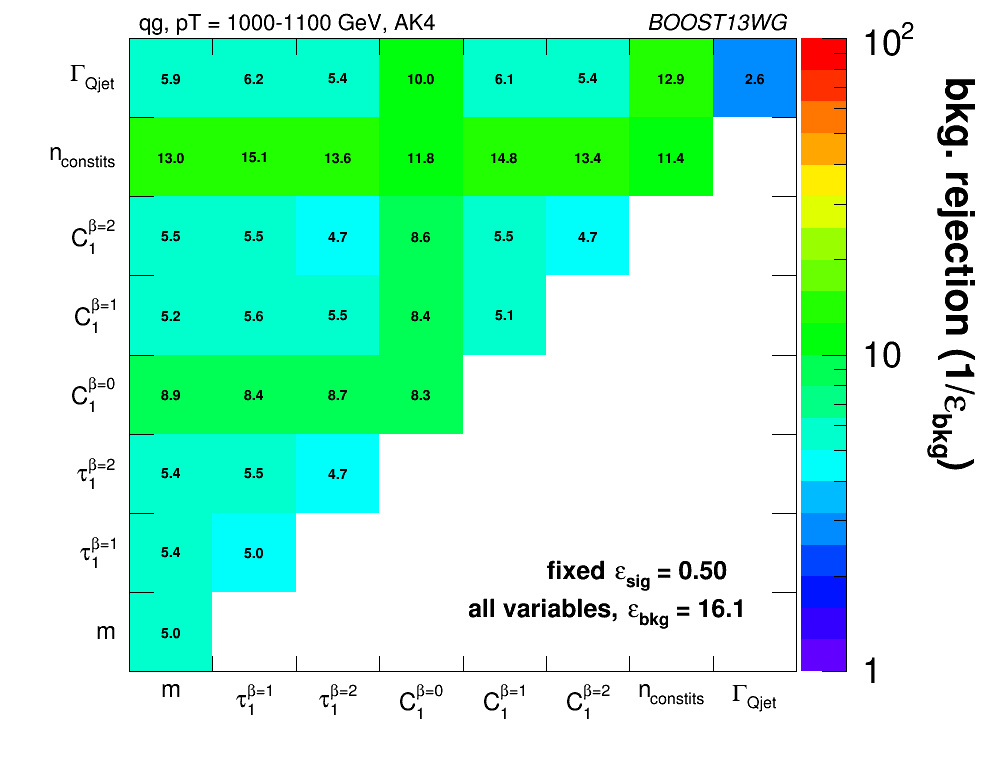
\includegraphics[width=0.32\textwidth]{./Figures/QGTagging/pT1000/AKtR04/effBkg2D.png}
%\includegraphics[width=0.4\textwidth]{./Figures/QGTagging/pT1000/AKtR04/Rocs_1D_single.png}\\
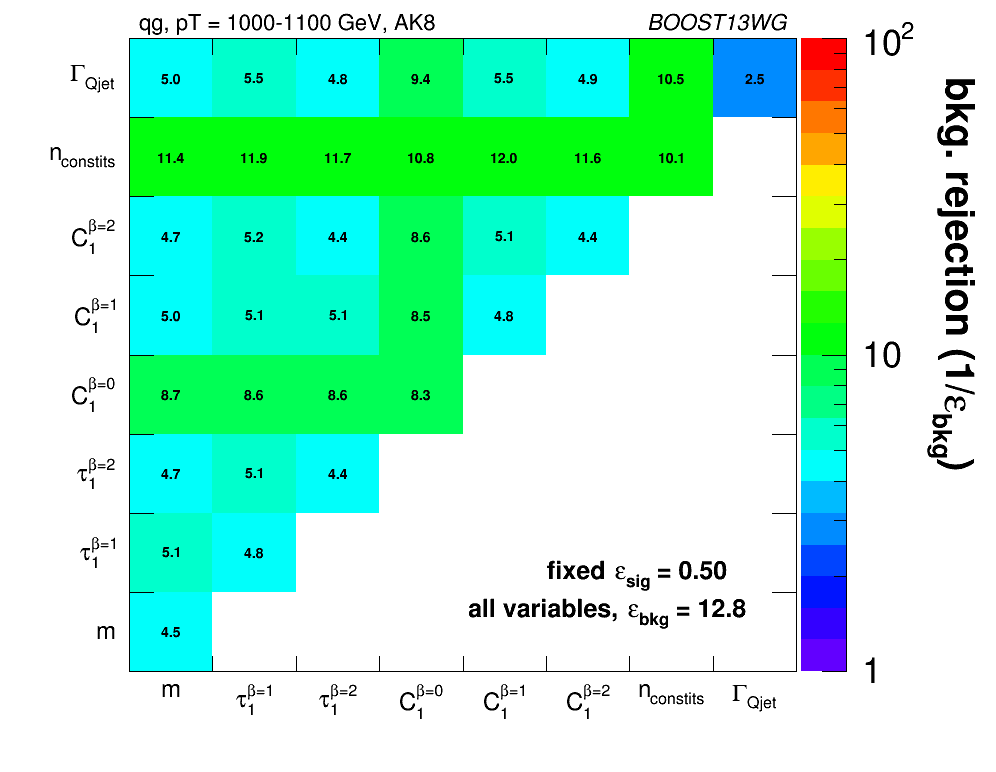
\includegraphics[width=0.32\textwidth]{./Figures/QGTagging/pT1000/AKtR08/effBkg2D.png}
%\includegraphics[width=0.4\textwidth]{./Figures/QGTagging/pT1000/AKtR08/Rocs_1D_single.png}\\
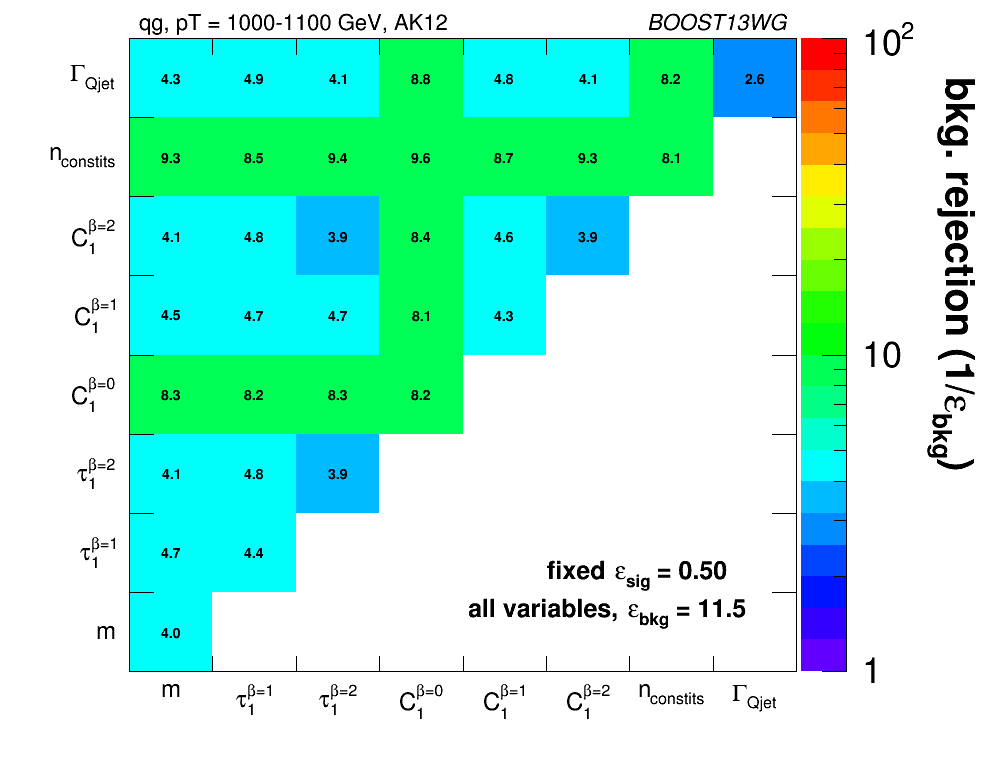
\includegraphics[width=0.32\textwidth]{./Figures/QGTagging/pT1000/AKtR12/effBkg2D.png}
%\includegraphics[width=0.4\textwidth]{./Figures/QGTagging/pT1000/AKtR12/Rocs_1D_single.png}\\
\caption{Gluon rejection defined as $1/\epsilon_{\rm gluon}$ when using each 2-variable combination 
as a tagger with 50\% acceptance for quark jets. Results are shown for jets with $\pt=1-1.2 \TeV$ and
for (left) $R=0.4$; (centre) $R=0.8$; (right) $R=1.2$. The rejection obtained with a tagger that uses all variables is also shown
in the plots. }
\label{fig:qg_pt1000_comb}
\end{center}
\end{figure*}
As already observed in the previous section, $n_{\rm constits}$ is the most powerful single variable and
$\C{1}{\beta=0}$ follows closely. However, the gains are largely correlated; the combined performance of $n_{\rm constits}$ and $\C{1}{\beta=0}$ is generally poorer than combinations of $n_{\rm constits}$ with other jet substructure observables, such as $\tau_1$. Interestingly, in spite of the high correlation between $n_{\rm constits}$ and $\C{1}{\beta=0}$, the two-variable combinations of $n_{\rm constits}$ generally fare worse than two-variable combinations with $\C{1}{\beta=0}$ . In particular,
the combinations of $\tau^{\beta=1}_1$ or $\C{1}{\beta=1}$ with $n_{\rm constits}$ are capable of 
getting very  close to the rejection achievable through the use of all variables for $R=0.4$ and $R=0.8$.


 Tagger performance is generally better at small $R$. 
The overall loss in performance
with increasing $R$ can be seen in most single variables we study; this is expected, since more of the parton radiation is captured in the jet and more contamination from underlying event occurs, suppressing the differences between $q$/$g$ jets. 
The principal exceptions are $\C{1}{\beta=0}$ and 
the Q-jet mass volatility, which are both quite resilient to increasing $R$. For $\C{1}{\beta=0}$, this is due to the fact that the exponent on $\Delta R$ is zero, and so soft radiation at the periphery of the jet does not substantially change the distribution; as a result, the performance is largely independent of $R$.  Similarly, the soft radiation distant from the jet centre will be vetoed during pruning regardless of the cluster sequence, and so the $R$-dependence of $\Gamma_{\rm Qjet}$ is not significant.   ({\bf BS: Check my logic?}) Their combination, however, does perform slightly worse at larger $R$. ({\bf BS: I don't understand this, but it is a $\sim10\%$ effect, so maybe not too significant?}).
By contrast, $\tau_1^{(\beta=2)}$ and $\C{1}{\beta=2}$
are particularly sensitive to increasing R since, for $\beta=2$,
 large-angle emissions are given a larger weight. 

These observations are qualitatively similar across all ranges of $\pt$. Quantitatively, however,
there is a loss of rejection power for the taggers made of a combination of variables as the $\pt$ decreases. 
This can be observed in Fig.~\ref{fig:qg_akt4_comb} for anti-$\kT$ R=0.4 jets of different $\pt$s. 
\begin{figure*}
\begin{center}
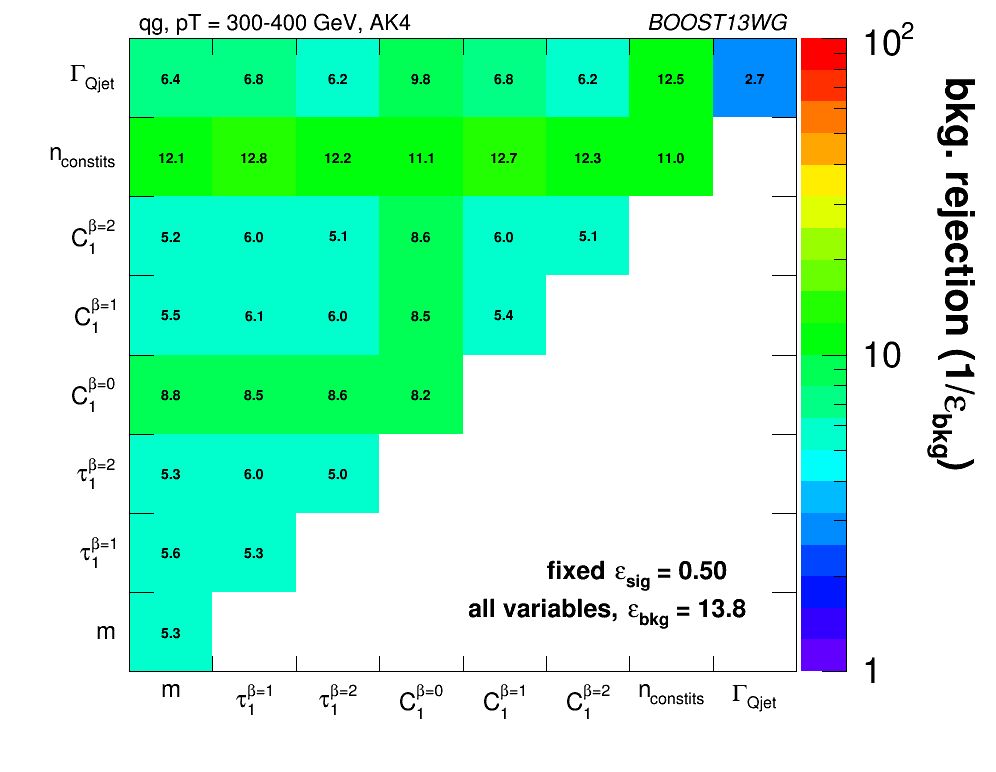
\includegraphics[width=0.32\textwidth]{./Figures/QGTagging/pT300/AKtR04/effBkg2D.png}
%\includegraphics[width=0.4\textwidth]{./Figures/QGTagging/pT1000/AKtR04/Rocs_1D_single.png}\\
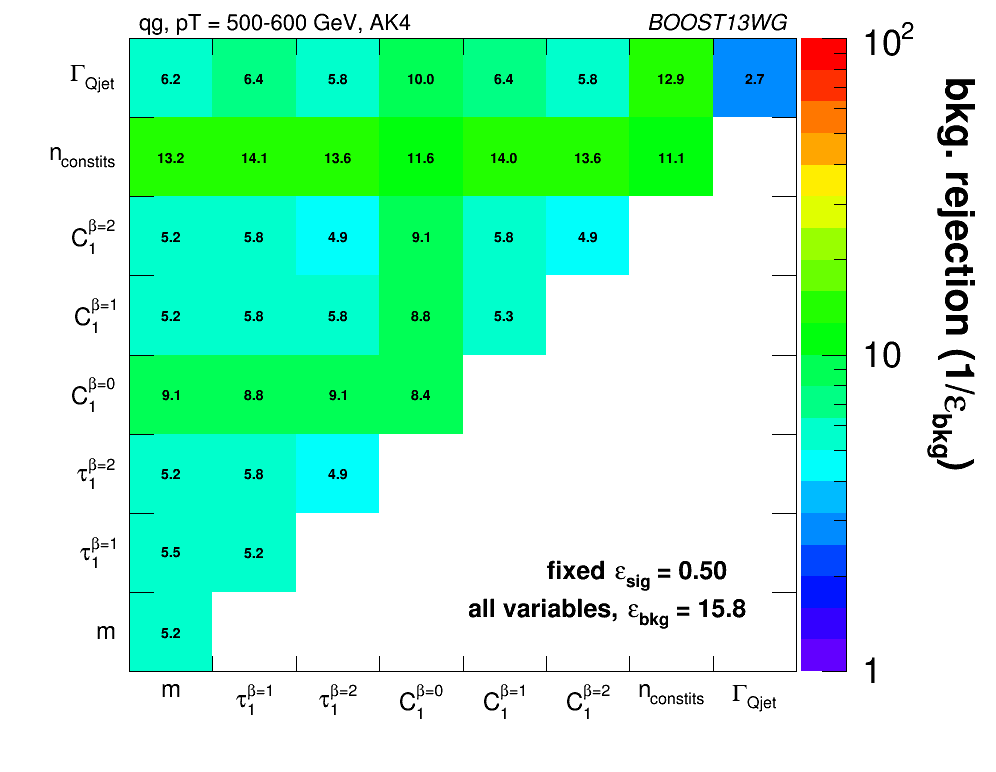
\includegraphics[width=0.32\textwidth]{./Figures/QGTagging/pT500/AKtR04/effBkg2D.png}
%\includegraphics[width=0.4\textwidth]{./Figures/QGTagging/pT1000/AKtR08/Rocs_1D_single.png}\\
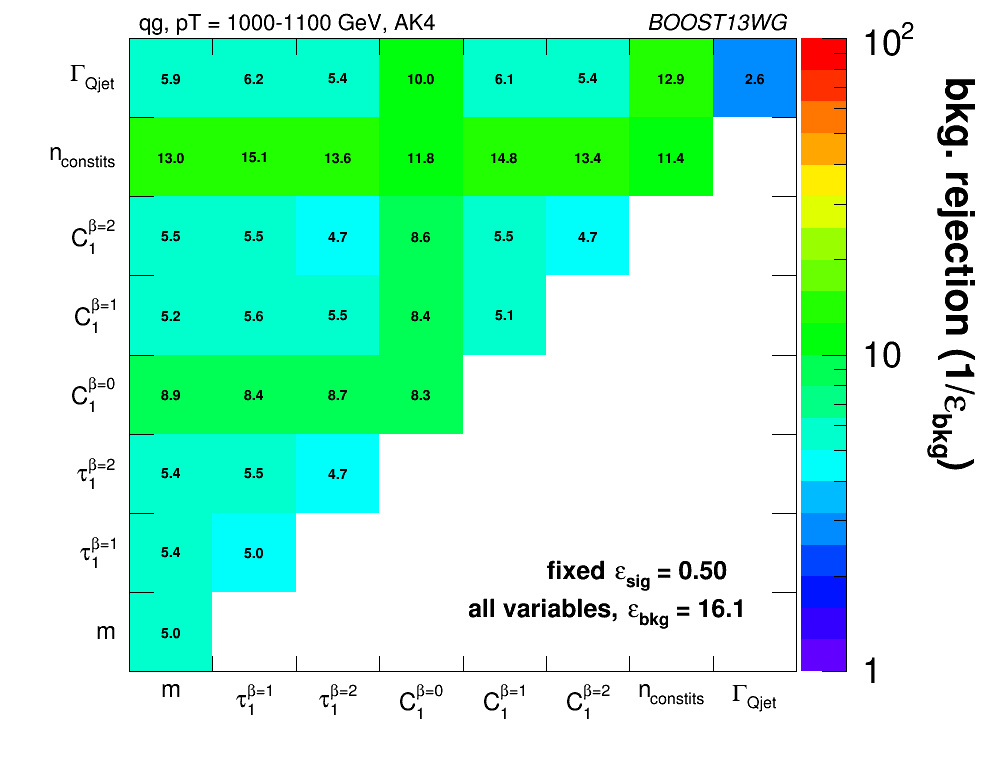
\includegraphics[width=0.32\textwidth]{./Figures/QGTagging/pT1000/AKtR04/effBkg2D.png}
%\includegraphics[width=0.4\textwidth]{./Figures/QGTagging/pT1000/AKtR12/Rocs_1D_single.png}\\
\caption{Gluon rejection defined as $1/\epsilon_{\rm gluon}$ when using each 2-variable combination 
as a tagger with 50\% acceptance for quark jets. Results are shown for R=0.4 jets with $\pt=300-400 \GeV$, 
$\pt=500-600 \GeV$ and $\pt=1-1.2 \TeV$. The rejection obtained with a tagger that uses all variables is also shown
in the plots. }
\label{fig:qg_akt4_comb}
\end{center}
\end{figure*}
Clearly, most single variables retain their gluon rejection potential at lower $\pt$. However, when combined
with other variables, the highest performing pairwise combinations lose ground with respect to other pairwise 
combinations. This is also reflected in the rejection of the tagger that uses a combination of all variables, which
is lower at lower $\pt$s. {\bf [do we understand this?]} ({\bf BS: This is a bit of a guess, but could it be that there is typically less radiation for low $\pt$, and so you're more sensitive to fluctuations; since you have less access to information, combinations of observables perform less well than at high $\pt$.})


%\subsection{QJets Volatility and $\ptd$ ($\C{1}{\beta=0}$)}

%Simple explanation of correlation, or why does combining volatility and $\ptd$ improve quark versus gluon discrimination.  $\ptd$ ($\C{1}{\beta=0}$) takes small (large) values for a jet with near-democratic energy sharing between particles and large (small) values when the energy of the jet is contained in a few particles.  Because we expect gluons to radiate more particles, we expect that $\ptd_g<\ptd_q$ (or ${\C{1}{\beta=0}}_g>{\C{1}{\beta=0}}_q$).  Now, we expect the volatility of gluon jets to be in general smaller than that of quark jets because there is a greater probability (by a factor of about $C_A/C_F=9/4$) that there was a relatively hard emission in a jet that is not groomed away.  By measuring both volatility and $\ptd$, we are sensitive to both regions of phase space: where a relatively hard emission dominates the mass of the jet as well as the region where many soft emissions set the jet mass.
